\documentclass[12pt,a4paper,oneside]{report}

% --- Pacotes Fundamentais ---
\usepackage[utf8]{inputenc}
\usepackage[T1]{fontenc}
\usepackage[english]{babel}

% Renomeação manual de termos canônicos para Português (padrão ABNT / UEA)
\addto\captionsenglish{
    \renewcommand{\contentsname}{Sumário}
    \renewcommand{\listfigurename}{Lista de Figuras}
    \renewcommand{\listtablename}{Lista de Tabelas}
    \renewcommand{\bibname}{Referências Bibliográficas}
    \renewcommand{\chaptername}{Capítulo}
    \renewcommand{\appendixname}{Apêndice}
    \renewcommand{\figurename}{Figura}
    \renewcommand{\tablename}{Tabela}
}

\usepackage{times} % Tipografia Times New Roman / padrão acadêmico
\usepackage{geometry}
\geometry{
    a4paper,
    top=3.0cm,
    left=3.0cm,
    bottom=2.0cm,
    right=2.0cm
}
\usepackage{setspace}
\onehalfspacing % Espaçamento 1.5 entre linhas

% --- Pacotes de Matemática, Figuras e Tabelas ---
\usepackage{amsmath,amssymb,amsfonts}
\usepackage{graphicx}
\usepackage{booktabs}
\usepackage{tabularx}
\usepackage{caption}
\usepackage{subcaption}
\usepackage{xcolor}
\usepackage{enumitem}
\usepackage{float}
\usepackage{placeins}
\usepackage{listings}
\lstset{
    basicstyle=\ttfamily\scriptsize,
    breaklines=true,
    breakatwhitespace=true,
    frame=single,
    showstringspaces=false,
    columns=flexible,
    keepspaces=true,
    tabsize=2,
    xleftmargin=1.0em,
    xrightmargin=1.0em
}
\usepackage{tikz}
\usetikzlibrary{shapes.geometric, arrows, positioning, calc, fit, backgrounds}
\usepackage{pgfplots}
\pgfplotsset{compat=1.18}

% --- Títulos e Cabeçalhos ---
\usepackage{titlesec}
\titleformat{\chapter}[hang]{\normalfont\LARGE\bfseries}{\thechapter\hspace{10pt}|\hspace{10pt}}{0pt}{\LARGE\bfseries}
\titlespacing*{\chapter}{0pt}{-10pt}{20pt}
\titleformat{\section}{\normalfont\Large\bfseries}{\thesection}{1em}{}
\titleformat{\subsection}{\normalfont\large\bfseries}{\thesubsection}{1em}{}
\titleformat{\subsubsection}{\normalfont\normalsize\bfseries}{\thesubsubsection}{1em}{}

\usepackage{fancyhdr}
\setlength{\headheight}{15pt}
\pagestyle{fancy}
\fancyhf{}
\rhead{\thepage}
\renewcommand{\headrulewidth}{0pt}

% --- Citações e Links ---
\usepackage{cite}
\usepackage{url}
\usepackage{hyperref}
\hypersetup{
    colorlinks=true,
    linkcolor=black,
    citecolor=blue!70!black,
    urlcolor=blue!70!black
}

\begin{document}

% ==========================================
% ELEMENTOS PRÉ-TEXTUAIS
% ==========================================
\pagenumbering{roman}

% --- CAPA ---
\begin{titlepage}
\begin{center}
    {\large \textbf{UNIVERSIDADE DO ESTADO DO AMAZONAS -- UEA}}\\[0.2cm]
    {\large \textbf{ESCOLA SUPERIOR DE TECNOLOGIA -- EST}}\\[0.2cm]
    {\large \textbf{CURSO DE BACHARELADO EM SISTEMAS DE INFORMAÇÃO}}\\[3.5cm]

    {\large \textbf{JOÃO LUCAS NORONHA DE CASTRO}}\\[3.5cm]

    {\Large \textbf{AVALIAÇÃO DE MODELOS DE LINGUAGEM DE GRANDE ESCALA NA GERAÇÃO DINÂMICA DE DIÁLOGOS PARA PERSONAGENS NÃO JOGÁVEIS EM JOGOS DE INVESTIGAÇÃO}}\\[4.0cm]

    \vfill
    {\large \textbf{Manaus -- AM}}\\[0.2cm]
    {\large \textbf{2026}}
\end{center}
\end{titlepage}

% --- FOLHA DE ROSTO ---
\newpage
\begin{center}
    {\large \textbf{JOÃO LUCAS NORONHA DE CASTRO}}\\[4.0cm]

    {\Large \textbf{AVALIAÇÃO DE MODELOS DE LINGUAGEM DE GRANDE ESCALA NA GERAÇÃO DINÂMICA DE DIÁLOGOS PARA PERSONAGENS NÃO JOGÁVEIS EM JOGOS DE INVESTIGAÇÃO}}\\[2.5cm]

    \hfill
    \begin{minipage}{0.55\textwidth}
        \linespread{1.1}\selectfont
        \small
        Monografia de Trabalho de Conclusão de Curso (TCC II) apresentada à Escola Superior de Tecnologia da Universidade do Estado do Amazonas (EST/UEA) como requisito parcial para a obtenção do título de Bacharel em Sistemas de Informação.\\[0.5cm]
        \textbf{Orientador:} Prof. Dr. Luis Cuevas Rodriguez
    \end{minipage}\\[4.0cm]

    \vfill
    {\large \textbf{Manaus -- AM}}\\[0.2cm]
    {\large \textbf{2026}}
\end{center}

% --- FOLHA DE APROVAÇÃO ---
\newpage
\begin{center}
    {\large \textbf{JOÃO LUCAS NORONHA DE CASTRO}}\\[1.5cm]

    {\large \textbf{AVALIAÇÃO DE MODELOS DE LINGUAGEM DE GRANDE ESCALA NA GERAÇÃO DINÂMICA DE DIÁLOGOS PARA PERSONAGENS NÃO JOGÁVEIS EM JOGOS DE INVESTIGAÇÃO}}\\[1.5cm]

    \hfill
    \begin{minipage}{0.55\textwidth}
        \linespread{1.1}\selectfont
        \small
        Monografia defendida e aprovada perante a Banca Examinadora do Curso de Sistemas de Informação da Escola Superior de Tecnologia da Universidade do Estado do Amazonas (EST/UEA).\\[0.3cm]
        \textbf{Nota Obtida:} \underline{\hspace{2.5cm}} pontos.\\[0.3cm]
        \textbf{Data da Defesa:} \underline{\hspace{1cm}} / \underline{\hspace{1cm}} / 2026.
    \end{minipage}\\[1.5cm]

    \textbf{BANCA EXAMINADORA}\\[1.5cm]

    \rule{0.75\textwidth}{0.5pt}\\
    \textbf{Prof. Dr. Luis Cuevas Rodriguez} -- Orientador\\
    Universidade do Estado do Amazonas (UEA)\\[1.2cm]

    \rule{0.75\textwidth}{0.5pt}\\
    \textbf{Prof. Dr. [Nome do Avaliador 1]} -- Examinador Interno\\
    Universidade do Estado do Amazonas (UEA)\\[1.2cm]

    \rule{0.75\textwidth}{0.5pt}\\
    \textbf{Prof. Dr. [Nome do Avaliador 2]} -- Examinador Externo / Interno\\
    Universidade do Estado do Amazonas (UEA)
\end{center}

% --- DEDICATÓRIA E AGRADECIMENTOS ---
\newpage
\chapter*{Agradecimentos}
\addcontentsline{toc}{chapter}{Agradecimentos}

Agradeço à minha família pelo apoio incondicional ao longo de toda a minha formação universitária. 

Ao meu orientador, Prof. Dr. Luis Cuevas Rodriguez, pela orientação precisa, paciência e incentivo constante durante a concepção e desenvolvimento desta pesquisa.

Aos colegas do curso de Sistemas de Informação da Universidade do Estado do Amazonas (UEA), pelas trocas de experiências, colaboração técnica e companheirismo durante esta jornada acadêmica.

A todos que direta ou indiretamente contribuíram para a realização deste trabalho.

\newpage
\chapter*{Epígrafe}
\addcontentsline{toc}{chapter}{Epígrafe}
\vspace*{14cm}
\hfill
\begin{minipage}{0.6\textwidth}
\textit{''Interactive narrative is not about the author dictating every branch, but creating intelligent worlds where player agency and emergent stories coexist seamlessly.''}
\vspace{0.3cm}
\hfill -- Mark O. Riedl
\end{minipage}

% --- RESUMO ---
\newpage
\chapter*{Resumo}
\addcontentsline{toc}{chapter}{Resumo}
\noindent Modelos de Linguagem de Grande Escala (\textit{Large Language Models} - LLMs) e Modelos Compactos (\textit{Small Language Models} - SLMs) representam uma alternativa arquitetural promissora para superar a rigidez e a explosão combinatória das tradicionais árvores de diálogo em jogos digitais, especialmente no gênero de dedução e mistério. No entanto, sua natureza estocástica introduz vulnerabilidades críticas de consistência espaço-temporal e suscetibilidade à quebra de persona sob pressão investigativa. Esta pesquisa desenvolve e avalia uma arquitetura híbrida de \textit{Agentic RAG} com fragmentação temporal dinâmica (\textit{Dynamic Chunking}) integrada ao motor gráfico Unity e executada localmente via framework Neo Cortex e plataforma Ollama. Submeteu-se uma bateria padronizada de 50 perguntas de inquérito sob estresse a quatro arquiteturas de modelos (Gemma-2-9b-it, Qwen-2.5-7b, Llama-3.1-8b e DeepSeek-R1-8b), auditando o desempenho pelo framework RAGAS com juiz sintético GPT-4o. Os resultados demonstram que o mecanismo de triagem e chunking alcançou precisão e recuperação de contexto perfeitas (1,00), validando a arquitetura de recuperação. Entre os modelos geradores, Gemma-2-9b-it obteve a maior fidelidade factual (0,38) e relevância (0,60), enquanto Llama-3.1-8b destacou-se pela riqueza de atuação dramática à custa de precisão factual (0,30). O DeepSeek-R1-8b apresentou instabilidade severa sob baixas temperaturas, quebrando a quarta parede. Conclui-se que a simulação robusta de NPCs exige uma abordagem de engenharia narrativa que desacople a recuperação de contexto da síntese dialógica, estabelecendo parâmetros para a adoção sustentável de IA generativa em hardware local de jogos.

\vspace{0.8cm}
\noindent \textbf{Palavras-chave:} Modelos de Linguagem, Personagens Não Jogáveis, Jogos de Investigação, Agentic RAG, Consistência Espaço-Temporal, RAGAS.

% --- ABSTRACT ---
\newpage
\chapter*{Abstract}
\addcontentsline{toc}{chapter}{Abstract}
\noindent Large Language Models (LLMs) and Small Language Models (SLMs) offer a transformative architectural approach to overcoming the authorial bottleneck and combinatorial explosion of static dialogue trees in digital games, particularly within the mystery and detective genre. However, their probabilistic nature introduces severe vulnerabilities in spatiotemporal consistency, character hallucination, and persona derailment under rigorous cross-examination. This research develops and evaluates a hybrid Agentic RAG architecture featuring Dynamic Temporal Chunking, seamlessly integrated into the Unity engine and executed locally via the Neo Cortex middleware and the Ollama runtime. A standardized stress-test suite of 50 investigative inquiries across five vulnerability categories was administered to four distinct models (Gemma-2-9b-it, Qwen-2.5-7b, Llama-3.1-8b, and DeepSeek-R1-8b), followed by automated evaluation using the RAGAS framework with GPT-4o as a synthetic judge. Experimental findings show that the routing and chunking pipeline achieved perfect Context Precision and Recall (1.00), validating the retrieval architecture. Among generators, Gemma-2-9b-it achieved superior factual faithfulness (0.38) and answer relevance (0.60), whereas Llama-3.1-8b exhibited rich dramatic embodiment accompanied by minor temporal drift (0.30 faithfulness). DeepSeek-R1-8b collapsed into algorithmic meta-responses when restricted by low temperatures. We conclude that robust NPC simulation requires decoupling factual retrieval from dramatic synthesis, establishing concrete architectural guidelines for edge-deployed generative dialogue in games.

\vspace{0.8cm}
\noindent \textbf{Keywords:} Large Language Models, Non-Player Characters, Investigation Games, Agentic RAG, Spatiotemporal Consistency, RAGAS.

% --- LISTAS ---
\newpage
\listoffigures
\addcontentsline{toc}{chapter}{\listfigurename}

\newpage
\listoftables
\addcontentsline{toc}{chapter}{\listtablename}

\newpage
\chapter*{Lista de Abreviaturas e Siglas}
\addcontentsline{toc}{chapter}{Lista de Abreviaturas e Siglas}
\begin{tabular}{ll}
API & \textit{Application Programming Interface} (Interface de Programação de Aplicações) \\
CRISP-DM & \textit{Cross-Industry Standard Process for Data Mining} \\
GGUF & \textit{GPT-Generated Unified Format} \\
GUI & \textit{Graphical User Interface} (Interface Gráfica de Usuário) \\
IA & Inteligência Artificial \\
JSON & \textit{JavaScript Object Notation} \\
LLM & \textit{Large Language Model} (Modelo de Linguagem de Grande Escala) \\
NLI & \textit{Natural Language Inference} (Inferência em Linguagem Natural) \\
NLP / PLN & \textit{Natural Language Processing} / Processamento de Linguagem Natural \\
NPC & \textit{Non-Player Character} (Personagem Não Jogável) \\
OOC & \textit{Out of Character} (Fora do Personagem) \\
RAG & \textit{Retrieval-Augmented Generation} (Geração Aumentada por Recuperação) \\
RAGAS & \textit{Retrieval Augmented Generation Assessment} \\
ReAct & \textit{Reasoning and Acting} (Raciocínio e Ação) \\
SLM & \textit{Small Language Model} (Modelo de Linguagem Compacto) \\
UEA & Universidade do Estado do Amazonas \\
UI & \textit{User Interface} (Interface de Usuário) \\
UX & \textit{User Experience} (Experiência do Usuário) \\
VRAM & \textit{Video Random Access Memory} (Memória de Vídeo) \\
\end{tabular}

\newpage
\tableofcontents

% ==========================================
% ELEMENTOS TEXTUAIS
% ==========================================
\newpage
\pagenumbering{arabic}
\setcounter{page}{1}

\chapter{Introdução}
\label{cap:introducao}

\section{Contextualização e Cenário dos Jogos Digitais}
\label{sec:contextualizacao}

A indústria global de jogos digitais consolidou-se nas últimas décadas como um dos segmentos mais dinâmicos e lucrativos do entretenimento contemporâneo. De acordo com o relatório econômico da Newzoo \cite{newzoo2024games}, o mercado global de jogos movimentou aproximadamente 187,7 bilhões de dólares em 2024, alcançando uma audiência estimada em 3,42 bilhões de jogadores ativos no planeta. Esse volume financeiro supera expressivamente o faturamento anual somado das indústrias de cinema em bilheteria e música gravada, consolidando os jogos como a principal mídia interativa da cultura digital.

Paralelamente a essa massiva expansão de mercado, as expectativas do público consumidor por experiências mais profundas, mundos virtuais críveis e narrativas não lineares cresceram em ritmo acelerado. No entanto, para atender a essa demanda por sofisticação estética e dramática, a produção de títulos de grande escala (frequentemente denominados produções AAA) passou a exigir ciclos de desenvolvimento que rotineiramente ultrapassam cinco a oito anos, mobilizando equipes multidisciplinares com centenas de profissionais e orçamentos multimilionários \cite{schreier2017blood}.

A inflação dos custos de produção atingiu patamares críticos na indústria contemporânea. No início dos anos 2000, títulos de grande sucesso eram concluídos com orçamentos situados entre 10 e 25 milhões de dólares. Em contraste, produções recentes registram cifras alarmantes: a desenvolvedora polonesa CD Projekt Red divulgou oficialmente que o título \textit{Cyberpunk 2077} consumiu cerca de 316 milhões de dólares até o seu lançamento (174 milhões em desenvolvimento direto e 142 milhões em campanhas de marketing), ultrapassando a marca de 440 milhões de dólares de investimento total ao se contabilizarem as reformulações técnicas e a expansão \textit{Phantom Liberty} \cite{cdprojekt2023report}. De forma análoga, documentos corporativos da Sony e da Insomniac Games revelaram que o título \textit{Marvel's Spider-Man 2} exigiu mais de 315 milhões de dólares de orçamento, enquanto \textit{The Last of Us Part II}, da Naughty Dog, ultrapassou 220 milhões de dólares em custos diretos de engenharia e arte.

\begin{figure}[htbp]
\centering
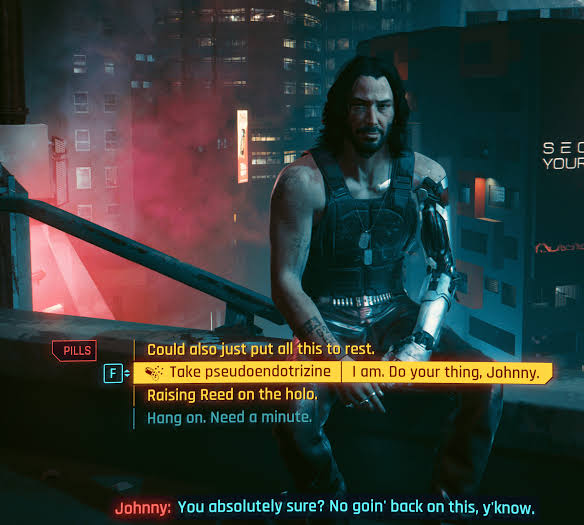
\includegraphics[width=0.78\textwidth]{figuras/dialogue_cyberpunk.jpg}
\caption{Interface contemporânea de diálogo em produções AAA (exemplo em \textit{Cyberpunk 2077}), evidenciando a mecânica de seleção manual de opções pré-definidas.}
\label{fig:cyberpunk_dialogo}
\end{figure}

Apesar desses investimentos monumentais, a forma fundamental como os jogadores interagem verbalmente com os habitantes desses mundos virtuais permanece essencialmente a mesma há décadas. Conforme ilustrado na Figura \ref{fig:cyberpunk_dialogo}, mesmo em produções que demandaram centenas de milhões de dólares, o jogador depara-se com uma interface baseada em um menu estático com poucas alternativas de texto pré-escritas.

Historicamente, a interatividade narrativa e o comportamento verbal de Personagens Não Jogáveis (\textit{Non-Player Characters}, NPCs) têm sido estruturados sobre arquiteturas de árvores de diálogo determinísticas e máquinas de estados finitos \cite{adams2014fundamentals}. Embora essas abordagens garantam aos autores e desenvolvedores um controle absoluto sobre a consistência textual e o fluxo da história, elas impõem barreiras intransponíveis à imersão e à agência do jogador. Sob esse paradigma clássico, o jogador é confinado a escolher entre réplicas textuais pré-concebidas; esgotadas as opções do roteiro, o personagem inevitavelmente retorna a ciclos de respostas repetitivas ou declarações genéricas, quebrando a suspensão da descrença \cite{murray1997hamlet}.

\begin{figure}[htbp]
\centering
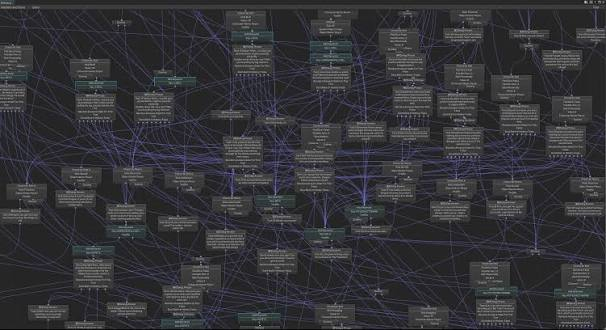
\includegraphics[width=0.82\textwidth]{figuras/arvore_dialogo_complexa.jpg}
\caption{Diagrama de ramificação massiva em uma árvore de diálogo tradicional, ilustrando a complexidade de rastreabilidade de caminhos e a explosão combinatória de autoria.}
\label{fig:arvore_complexa}
\end{figure}

O principal obstáculo intrínseco a essa abordagem de autoria manual é a denominada ``explosão combinatória''. Como exemplificado na Figura \ref{fig:arvore_complexa}, à medida que os roteiristas tentam oferecer ramificações reais de causa e efeito, a árvore de decisões multiplica-se exponencialmente a cada novo diálogo. Rastrear o impacto de centenas de nós interconectados gera um custo de autoria insustentável, forçando os estúdios a convergir os caminhos em nós comuns, resultando em uma sensação frequente de falsa agência ou linearidade disfarçada \cite{riedl2013interactive}.

Nesse cenário de gargalo produtivo, o Processamento de Linguagem Natural (PLN) e a Inteligência Artificial (IA) generativa emergem como alternativas estratégicas para transformar essa realidade. A emergência dos Modelos de Linguagem de Grande Escala (\textit{Large Language Models}, LLMs), fundamentados na arquitetura neural \textit{Transformer} \cite{vaswani2017attention}, viabiliza uma quebra histórica de paradigma. Ao permitirem que o fluxo de desenvolvimento transite da escrita exaustiva de ramificações para a parametrização de personas ricas em contexto \cite{shanahan2023role}, os modelos possibilitam a geração de diálogos em tempo real, nos quais o jogador pode formular perguntas em linguagem natural irrestrita.

\section{Formulação do Problema}
\label{sec:problema}

A superação das árvores estáticas de diálogo por meio de agentes gerativos encontra seu cenário de aplicação mais desafiador no gênero de jogos de mistério e dedução lógica \cite{fernandez2014introduction}. Em um jogo investigativo, a mecânica central (\textit{core gameplay loop}) centraliza-se no inquérito metódico de suspeitos, na coleta de testemunhos e na análise crítica de álibis, distinguindo-se fundamentalmente de dinâmicas baseadas em destreza motora ou combate. A literatura especializada classifica essa dinâmica como ``Linguagem de Processo'' (\textit{Process Language}), um regime interativo no qual o jogador atua como coautor do desdobramento narrativo \cite{fernandez2014introduction}. Para que essa mecânica funcione, o NPC deve sustentar rigorosamente suas restrições de papel, ocultar informações confidenciais de forma coerente e relatar eventos do passado com fidelidade factual inabalável.

No entanto, a inserção de modelos de linguagem generativos em ambientes que demandam determinismo factual revela vulnerabilidades intrínsecas à sua natureza probabilística. Os LLMs operam prevendo o próximo \textit{token} estatisticamente mais provável, o que acarreta o risco persistente de alucinações \cite{ji2023survey}. No contexto de simulação de personas (\textit{roleplay}), essa deficiência manifesta-se criticamente como ``alucinação de personagem'' (\textit{character hallucination}), em que o modelo inventa fatos ausentes do roteiro ou assume posturas contraditórias à sua identidade ficcional.

Em jogos de investigação, o impacto da alucinação de personagem é destrutivo. Se um suspeito afirmar falsamente ter presenciado uma cena em um horário em que se encontrava em outro cômodo, ou revelar detalhes que somente o assassino conheceria, a integridade de todo o mistério é violada. Esse erro de consistência espaço-temporal invalida a dedução lógica do jogador \cite{ahn2024timechara}. Além disso, modelos compactos executados em hardware local sofrem frequentemente do fenômeno de perda de contexto (\textit{Lost in the Middle}) quando submetidos a históricos extensos de conversa \cite{liu2024lost}, ou quebram a persona respondendo de forma metalinguística como assistentes virtuais (\textit{Out-of-Character}, OOC).

\subsection{O Abismo Econômico dos Custos Recorrentes por Token}
\label{subsec:custo_tokens_problema}

Além das vulnerabilidades lógicas, existe uma barreira econômica fundamental que inviabiliza o uso ingênuo de APIs comerciais proprietárias na nuvem (tais como OpenAI GPT-4o ou Anthropic Claude) em jogos de entretenimento comercial.

Os jogos para computadores e consoles são historicamente comercializados sob o modelo de compra única (\textit{Buy-to-Play}, B2P), no qual o consumidor paga um valor fixo (por exemplo, 20 a 70 dólares) e obtém direito irrestrito de jogabilidade por dezenas ou centenas de horas. Nesse modelo de negócios, o estúdio possui receita marginal zero após a venda da cópia. 

Entretanto, as APIs proprietárias de inteligência artificial cobram continuamente por volume de \textit{tokens} trafegados tanto na entrada (\textit{prompt}) quanto na saída (\textit{completion}). Em sessões investigativas densas, onde a cada turno é necessário enviar o histórico de mensagens acumulado, o perfil psicológico e o roteiro do caso, cada requisição consome facilmente entre 3.000 e 6.000 \textit{tokens}. Se um estúdio independente comercializar 50.000 cópias de um jogo e cada jogador realizar uma média modesta de 250 turnos de inquérito ao longo da campanha, o sistema processará mais de 12,5 milhões de chamadas de API, acumulando dezenas de bilhões de \textit{tokens}. Com as tarifas vigentes de modelos de fronteira na nuvem, a fatura de servidores consumiria centenas de milhares de dólares, superando rapidamente a própria margem de lucro líquida obtida com as vendas do jogo. 

Esse descompasso financeiro cria um incentivo perverso inaceitável para o desenvolvedor: quanto mais o jogador se engaja com o jogo e conversa com os personagens, maior é o prejuízo operacional imposto ao estúdio. Portanto, a transição para Modelos Compactos (\textit{Small Language Models}, SLMs) executados diretamente no hardware de borda do usuário final (\textit{edge computing}), com custo marginal estritamente nulo por turno, constitui a única via economicamente sustentável para democratizar NPCs generativos na indústria independente.

\section{Questão de Pesquisa e Hipótese}
\label{sec:questoes_pesquisa}

Diante da problemática exposta, formula-se a seguinte questão norteadora da pesquisa:

\begin{quote}
\textit{Como uma arquitetura híbrida de Agentic RAG com fragmentação temporal dinâmica influencia a consistência espaço-temporal, a fidelidade factual e a estabilidade de persona em NPCs conduzidos por modelos de linguagem compactos executados localmente em jogos de investigação?}
\end{quote}

A hipótese central deste trabalho estabelece que a substituição de \textit{prompts} estáticos completos (\textit{Full Prompt}) por um mecanismo de triagem autônoma (\textit{Agentic RAG}) com fragmentação dinâmica do cronograma factual reduz o ruído informacional na janela de contexto, mitigando alucinações de personagem e permitindo que modelos compactos (entre 7 e 9 bilhões de parâmetros) atinjam níveis satisfatórios de fidelidade factual sem sacrificar a expressividade narrativa da persona, viabilizando economicamente a execução local com custo nulo de infraestrutura em nuvem.

\section{Objetivos}
\label{sec:objetivos}

Para responder à questão norteadora e validar a hipótese proposta, definem-se os seguintes objetivos:

\subsection{Objetivo Geral}
Desenvolver, integrar e avaliar comparativamente uma arquitetura híbrida de \textit{Agentic RAG} com fragmentação temporal dinâmica para a geração em tempo real de diálogos investigativos com NPCs, analisando a consistência espaço-temporal e a resiliência de diferentes modelos de linguagem de porte intermediário executados em ambiente computacional local.

\subsection{Objetivos Específicos}
\begin{enumerate}[label=\roman*.]
    \item Projetar e estruturar o cenário investigativo ficcional e a persona de inquérito (``Alberto Castelo''), formalizando seus atributos em dados estruturados (JSON) segregados em perfil biográfico, cronograma horário e grafo de relacionamentos;
    \item Implementar o ambiente lúdico interativo utilizando o motor gráfico Unity, estabelecendo a comunicação assíncrona com os modelos de linguagem locais gerenciados pela plataforma Ollama através do middleware Neo Cortex;
    \item Conceber e integrar o pipeline de \textit{Agentic RAG} baseado no paradigma ReAct (\textit{Reasoning and Acting}), incorporando o algoritmo de fragmentação dinâmica (\textit{Dynamic Chunking}) para despacho seletivo de blocos horários;
    \item Elaborar uma bateria experimental padronizada de 50 perguntas de inquérito sob estresse, categorizadas em cinco dimensões de vulnerabilidade: filtro de falsa informação, teste de direcionamento, consciência cronológica, resistência a evidências falsas e confronto direto de motivo;
    \item Avaliar quantitativamente o desempenho dos modelos Gemma-2-9b-it, Qwen-2.5-7b, Llama-3.1-8b e DeepSeek-R1-8b por meio do framework RAGAS com juiz sintético GPT-4o, analisando métricas de fidelidade factual, relevância e precisão de recuperação de contexto;
    \item Traçar o perfil comportamental e qualitativo individual de cada arquitetura avaliada, fornecendo diretrizes de engenharia de contexto para desenvolvedores de jogos digitais;
    \item Delinear e formalizar o protocolo experimental de validação ecológica com jogadores humanos na Universidade do Estado do Amazonas (UEA), definindo instrumentos psicométricos (módulo GEQ e escala SUS) para correlacionar a fidelidade computacional com a experiência de imersão e agência do usuário.
\end{enumerate}

\section{Justificativa e Relevância}
\label{sec:justificativa}

A relevância desta pesquisa fundamenta-se em três pilares interconectados:

\begin{itemize}
    \item \textbf{Relevância Científica:} Contribui para a literatura em Processamento de Linguagem Natural aplicada a sistemas interativos, investigando o comportamento de modelos de linguagem abertos em tarefas de simulação sob pressão inquisitiva adversária. Adicionalmente, discute criticamente a adequação de frameworks consolidados de avaliação (RAGAS) quando aplicados ao domínio de dramatização lúdica;
    \item \textbf{Relevância Tecnológica e Econômica:} Demonstra a viabilidade prática da execução de agentes inteligentes autônomos inteiramente em hardware de borda (\textit{edge computing} em computadores pessoais), eliminando as faturas recorrentes de APIs comerciais em nuvem e garantindo soberania de dados, baixa latência e viabilidade financeira definitiva para estúdios independentes;
    \item \textbf{Relevância para a Indústria de Jogos:} Oferece aos designers narrativos uma metodologia concreta de parametrização e controle contextual, reduzindo a complexidade combinatória inerente à autoria de árvores de diálogo sem abrir mão da agência do usuário.
\end{itemize}

\section{Estrutura da Monografia}
\label{sec:estrutura}

A presente monografia encontra-se estruturada em sete capítulos, organizados da seguinte forma:

O \textbf{Capítulo \ref{cap:introducao}} contextualizou o tema com dados econômicos da indústria, delimitou o problema de pesquisa e a barreira financeira de APIs, definiu as hipóteses e enumerou os objetivos gerais e específicos.

O \textbf{Capítulo \ref{cap:referencial}} apresenta o referencial teórico que alicerça o trabalho, discutindo a narrativa interativa em jogos, os fundamentos de LLMs e SLMs, técnicas de RAG e ReAct, as taxonomias de alucinação e os frameworks de avaliação automatizada baseados em LLM-as-a-Judge.

O \textbf{Capítulo \ref{cap:relacionados}} revisa os principais trabalhos relacionados na literatura, comparando abordagens seminais como os Agentes Generativos e estudos de caso comerciais com a proposta desta pesquisa por meio de uma matriz comparativa.

O \textbf{Capítulo \ref{cap:metodologia}} detalha a metodologia de pesquisa baseada no modelo CRISP-DM, a concepção do mistério ficcional e da Fase 1, a taxonomia da bateria de 50 testes de estresse e os protocolos experimental e humano.

O \textbf{Capítulo \ref{cap:implementacao}} documenta a engenharia de software da solução, abordando a integração Unity-NeoCortex-Ollama, os algoritmos de triagem e chunking dinâmico, e a infraestrutura de hardware utilizada.

O \textbf{Capítulo \ref{cap:resultados}} expõe os resultados empíricos, apresentando a análise quantitativa do RAGAS, o desacoplamento entre métricas de recuperação e geração, as transcrições qualitativas de inquérito, as hipóteses para testes humanos e o perfil comparativo dos modelos.

O \textbf{Capítulo \ref{cap:conclusao}} encerra a monografia com as considerações finais, a síntese das contribuições, as limitações metodológicas identificadas e os direcionamentos para trabalhos futuros.

\chapter{Referencial Teórico}
\label{cap:referencial}

Este capítulo estabelece a fundamentação teórica que sustenta o desenvolvimento e a avaliação experimental da pesquisa. A discussão divide-se em cinco tópicos essenciais: (i) as estruturas de narrativa interativa e o papel dos NPCs no gênero de investigação; (ii) os fundamentos de Modelos de Linguagem e as particularidades da inferência local de modelos compactos; (iii) os paradigmas de recuperação de informação, contrastando a injeção estática com a arquitetura \textit{Agentic RAG} e a fragmentação dinâmica; (iv) as taxonomias de alucinação de persona e inconsistência espaço-temporal; e (v) os métodos de avaliação automatizada baseados no paradigma \textit{LLM-as-a-Judge} e no framework RAGAS.

\section{Narrativa Interativa e Personagens Não Jogáveis (NPCs)}
\label{sec:ref_narrativa}

A interatividade em narrativas digitais difere fundamentalmente da experiência em mídias lineares, como a literatura e o cinema. Enquanto as mídias clássicas conduzem o receptor por um arco imutável de eventos, os jogos digitais operam sob a premissa da agência do usuário: a capacidade do jogador de executar ações intencionais que produzem efeitos observáveis no estado do mundo virtual \cite{murray1997hamlet,ryan2006interactive}. Na ludologia contemporânea, essa relação dialética entre regras de simulação e agência narrativa define a profundidade da imersão psicológica e da suspensão da descrença \cite{frasca2003simulation,bowman2012immersion}.

Historicamente, o comportamento e os diálogos de Personagens Não Jogáveis têm sido projetados através de abordagens determinísticas sustentadas por grafos direcionados e Máquinas de Estados Finitos (\textit{Finite State Machines}, FSM) \cite{adams2014fundamentals}. A Figura \ref{fig:arvore_dialogo_conceito} ilustra a topologia clássica de uma árvore de diálogo em jogos digitais.

\begin{figure}[htbp]
\centering
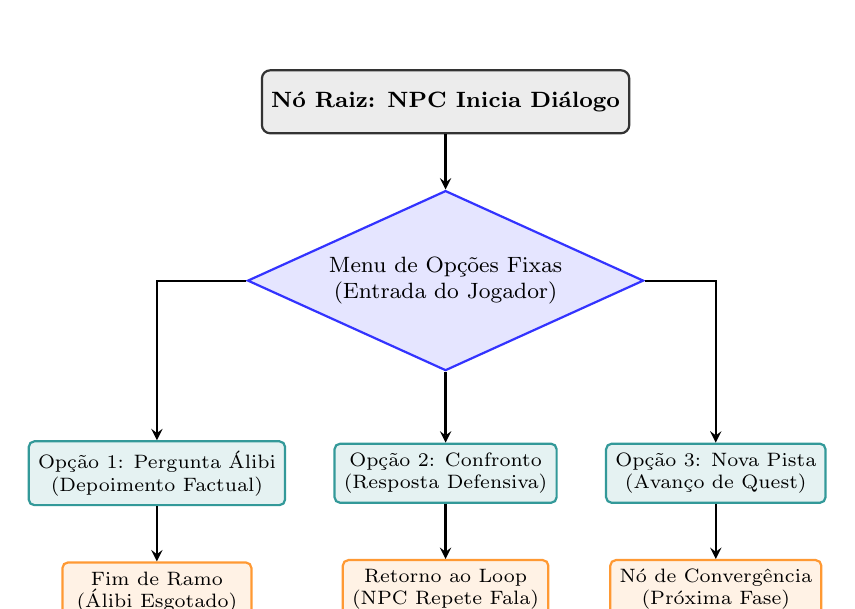
\begin{tikzpicture}[
    auto,
    node distance=1.1cm and 0.8cm,
    rootbox/.style={rectangle, rounded corners=3pt, draw=black!80, fill=gray!15, thick, minimum width=3.4cm, minimum height=0.8cm, align=center, font=\footnotesize\bfseries},
    decisionbox/.style={diamond, aspect=2.2, draw=blue!80, fill=blue!10, thick, minimum width=3.0cm, minimum height=0.8cm, align=center, font=\footnotesize},
    choicebox/.style={rectangle, rounded corners=2pt, draw=teal!80, fill=teal!10, thick, minimum width=2.6cm, minimum height=0.75cm, align=center, font=\scriptsize},
    leafbox/.style={rectangle, rounded corners=2pt, draw=orange!80, fill=orange!10, thick, minimum width=2.4cm, minimum height=0.7cm, align=center, font=\scriptsize},
    arr/.style={thick, ->, >=stealth}
]

    % Nós verticais principais
    \node (root) [rootbox] {Nó Raiz: NPC Inicia Diálogo};
    \node (dec) [decisionbox, below=0.7cm of root] {Menu de Opções Fixas\\(Entrada do Jogador)};

    % Três ramificações balanceadas
    \node (r2) [choicebox, below=0.9cm of dec] {Opção 2: Confronto\\(Resposta Defensiva)};
    \node (r1) [choicebox, left=0.6cm of r2] {Opção 1: Pergunta Álibi\\(Depoimento Factual)};
    \node (r3) [choicebox, right=0.6cm of r2] {Opção 3: Nova Pista\\(Avanço de Quest)};

    % Nós finais / convergência
    \node (leaf1) [leafbox, below=0.7cm of r1] {Fim de Ramo\\(Álibi Esgotado)};
    \node (leaf2) [leafbox, below=0.7cm of r2] {Retorno ao Loop\\(NPC Repete Fala)};
    \node (leaf3) [leafbox, below=0.7cm of r3] {Nó de Convergência\\(Próxima Fase)};

    % Conexões
    \draw [arr] (root) -- (dec);
    \draw [arr] (dec) -| (r1);
    \draw [arr] (dec) -- (r2);
    \draw [arr] (dec) -| (r3);

    \draw [arr] (r1) -- (leaf1);
    \draw [arr] (r2) -- (leaf2);
    \draw [arr] (r3) -- (leaf3);

\end{tikzpicture}
\caption{Estrutura conceitual de uma árvore de diálogo determinística tradicional.}
\label{fig:arvore_dialogo_conceito}
\end{figure}

Em uma árvore determinística, cada intervenção do jogador é limitada a um conjunto fechado de réplicas pré-concebidas pelos autores. Cada seleção conduz a um nó específico da estrutura hierárquica. O maior obstáculo inerente a essa abordagem é a denominada ``explosão combinatória'': à medida que se deseja proporcionar maior liberdade ao usuário, a quantidade de ramificações e caminhos alternativos necessários cresce exponencialmente. Como resultado, os custos de roteirização e dublagem tornam-se proibitivos para a indústria, forçando os desenvolvedores a concentrar escolhas em nós convergentes, gerando a sensação de ``falsa agência'' ou linearidade disfarçada \cite{riedl2013interactive}.

No gênero de investigação e mistério, a limitação da árvore estática compromete a mecânica fundamental do jogo. Conforme demonstrado por Fern{\'a}ndez-Vara \cite{fernandez2014introduction}, jogos investigativos demandam uma dinâmica de ``Linguagem de Processo'' (\textit{Process Language}), na qual a interrogação opera como uma ferramenta ativa de dedução abdutiva. Quando o jogador percebe que as opções do menu revelam previamente os tópicos a serem investigados, o desafio de dedução é esvaziado; o jogador é induzido a testar exaustivamente todas as opções da árvore mecânica até obter a pista, eliminando a autêntica investigação intelectual \cite{deng2024mindmap}.

\section{Modelos de Linguagem de Grande Escala e Inferência Local}
\label{sec:ref_llms}

Os Modelos de Linguagem de Grande Escala (LLMs) são redes neurais profundas pré-treinadas de forma auto-supervisionada sobre volumes massivos de dados textuais. A espinha dorsal dessa classe de modelos é a arquitetura \textit{Transformer}, introduzida por Vaswani et al. \cite{vaswani2017attention}, cujo mecanismo fundamental é o cálculo de atenção auto-atenciosa (\textit{self-attention}).

Dada uma sequência de representações vetoriais de entrada $X \in \mathbb{R}^{n \times d}$, onde $n$ é o comprimento da sequência e $d$ é a dimensão oculta, o mecanismo de atenção calcula projeções lineares de Consultas ($Q$), Chaves ($K$) e Valores ($V$):

\begin{equation}
Q = X W_Q, \quad K = X W_K, \quad V = X W_V
\label{eq:projecoes_qkv}
\end{equation}

\noindent onde $W_Q, W_K \in \mathbb{R}^{d \times d_k}$ e $W_V \in \mathbb{R}^{d \times d_v}$ são matrizes de parâmetros treináveis. O mapa de atenção ponderado é expresso pela formulação \textit{Scaled Dot-Product Attention}:

\begin{equation}
\text{Attention}(Q, K, V) = \text{softmax}\left(\frac{Q K^T}{\sqrt{d_k}}\right) V
\label{eq:scaled_dot_product}
\end{equation}

Essa formulação permite que o modelo pondere a relevância relativa de cada \textit{token} em relação a todos os demais elementos presentes na janela de contexto, superando as limitações de dependências temporais de longo alcance que afetavam redes neurais recorrentes anteriores (RNNs e LSTMs).

\subsection{O Dilema Arquitetural: APIs Proprietárias na Nuvem vs. Inferência Local em Borda}
\label{subsec:ref_custos_tokens}

A viabilização comercial de NPCs inteligentes em jogos digitais esbarra na arquitetura de execução dos modelos. Embora modelos proprietários de ponta (como GPT-4o e Claude 3.5 Sonnet) apresentem elevada capacidade de raciocínio, sua operação via APIs na nuvem impõe gargalos severos e frequentemente intransponíveis para estúdios de desenvolvimento de jogos:

\begin{itemize}
    \item \textbf{A Inviabilidade Econômica dos Custos Recorrentes por Token:} No modelo tradicional de comercialização de jogos (\textit{Buy-to-Play}), o usuário realiza o pagamento único pelo título e espera desfrutar de horas ilimitadas de conteúdo. Em contrapartida, provedores de IA na nuvem cobram por volume consumido:
    
    \begin{equation}
    C_{\text{total}} = \sum_{p=1}^{N_{\text{jogadores}}} \sum_{t=1}^{T_p} \left( c_{\text{in}} \cdot k_{\text{in}}^{(p,t)} + c_{\text{out}} \cdot k_{\text{out}}^{(p,t)} \right)
    \label{eq:custo_api}
    \end{equation}
    
    onde $c_{\text{in}}$ e $c_{\text{out}}$ representam as tarifas por milhão de \textit{tokens} de entrada e saída, e $k_{\text{in}}^{(p,t)}$ é a extensão do contexto enviado no turno $t$. Em sessões de inquérito investigativo denso, onde cada requisição concatena históricos de conversa e bases factuais (frequentemente entre 3.000 e 6.000 \textit{tokens}), uma base modesta de 50.000 jogadores ativos realizando 200 turnos cada demandará mais de 40 bilhões de \textit{tokens}. As faturas mensais de nuvem podem atingir centenas de milhares de dólares, consumindo integralmente a margem de receita do jogo e penalizando financeiramente o estúdio quanto maior for o engajamento de seus jogadores;
    \item \textbf{Latência de Rede e Quebra de Fluência Lúdica:} A dependência de servidores remotos introduz variações de latência de transporte (frequentemente de 2 a 5 segundos por interação), destruindo o ritmo natural da conversa face a face com o suspeito;
    \item \textbf{Privacidade, Soberania de Dados e Modo Offline:} A exigência de conexão ininterrupta à internet impede a execução do jogo em ambientes desconectados e expõe as conversas dos usuários a tráfego em servidores de terceiros.
\end{itemize}

Diante dessas restrições, a emergência de Modelos Compactos (\textit{Small Language Models}, SLMs), situados na faixa de 7 a 9 bilhões de parâmetros, destaca-se como a fronteira de aplicação mais promissora para jogos digitais \cite{cao2026task}. Tecnologias de quantização em pós-treinamento, especialmente o formato GGUF em 4 bits (\textit{e.g.}, Q4\_K\_M), reduzem substancialmente o uso de memória de vídeo (VRAM) e a banda de transferência de dados, viabilizando taxas de geração fluídas (acima de 25 \textit{tokens} por segundo) em placas de vídeo de consumo doméstico ou até mesmo em processadores centrais modernos. Plataformas de código aberto como o Ollama atuam como orquestradores eficientes para empacotamento, gerenciamento e inferência local dessas arquiteturas, fixando o custo marginal por turno em estritamente zero ($c_{\text{in}} = c_{\text{out}} = 0$).

\section{Engenharia de Contexto: De Naive RAG a Agentic RAG}
\label{sec:ref_rag}

Para que um modelo fundacional assuma a identidade de um personagem específico e respeite as regras de um roteiro ficcional, seu comportamento precisa ser condicionado via engenharia de \textit{prompt} e injeção de contexto \cite{shanahan2023role}.

A abordagem mais elementar consiste na injeção estática completa (\textit{Full Prompt}). Nesse método, toda a base de conhecimento do personagem (dados biográficos, cronograma completo de 24 horas, inventário e histórico de relações) é concatenada e enviada integralmente ao modelo a cada turno de conversação. Essa técnica gera problemas substanciais:

\begin{enumerate}
    \item \textbf{Saturação da Janela de Contexto e Custo Computacional:} A retransmissão de milhares de \textit{tokens} a cada pergunta do jogador eleva o processamento computacional da fase de pré-preenchimento (\textit{prefill phase}), elevando o tempo de resposta;
    \item \textbf{O Fenômeno \textit{Lost in the Middle}:} Conforme evidenciado por Liu et al. \cite{liu2024lost}, modelos baseados em atenção tendem a recuperar informações com alta precisão quando localizadas no início ou no fim do contexto, mas sofrem de degradação acentuada de recuperação quando os fatos relevantes encontram-se dispostos no centro de \textit{prompts} longos.
\end{enumerate}

Para superar essas fragilidades, a Geração Aumentada por Recuperação (\textit{Retrieval-Augmented Generation}, RAG) foi originalmente proposta por Lewis et al. \cite{lewis2020retrieval}. No RAG tradicional (\textit{Naive RAG}), uma base de documentos externos é dividida em blocos (\textit{chunks}), indexada via representações vetoriais (\textit{embeddings}) e consultada por similaridade de cosseno a cada interação do usuário. Embora eficaz para bases textuais abertas, o \textit{Naive RAG} demonstra rigidez para raciocínios temporais complexos, uma vez que a similaridade semântica direta frequentemente falha em capturar relações cronológicas precisas (ex: distinguir o que aconteceu às 08:30 versus 18:30).

\subsection{A Arquitetura Agentic RAG e o Paradigma ReAct}
Para solucionar as deficiências dos métodos estáticos e vetoriais em tarefas complexas de inquérito, adota-se nesta pesquisa o conceito de \textit{Agentic RAG}. Diferente do fluxo passivo de recuperação, um agente dotado de capacidade de raciocínio é encarregado de analisar a intenção do usuário antes de emitir a resposta final.

A base teórica dessa abordagem apoia-se no framework ReAct (\textit{Reasoning and Acting}), formulado por Yao et al. \cite{yao2023react}. O ReAct integra de forma sinérgica o raciocínio em linguagem natural (\textit{Thought}) com a execução de ações deliberadas (\textit{Action}), gerando um ciclo iterativo de resolução de problemas:

\begin{equation}
\text{Pensamento} \rightarrow \text{Ação} \rightarrow \text{Observação} \rightarrow \text{Conclusão}
\label{eq:ciclo_react}
\end{equation}

No contexto de jogos de investigação, o agente de triagem utiliza o ReAct para decompor a pergunta do detetive. Se o jogador indaga sobre um álibi matutino, o modelo raciocina: ``\textit{O jogador está questionando minhas ações durante a manhã; logo, devo requisitar apenas o bloco temporal correspondente ao início do dia}''. O agente então emite uma ação controlada que recupera exclusivamente o fragmento pertinente.

\subsection{Fragmentação Temporal Dinâmica (\textit{Dynamic Chunking})}
A técnica de fragmentação temporal dinâmica consiste em segmentar a linha do tempo do personagem em janelas discretas coerentes com a estrutura dramática do caso (ex: Manhã, Tarde e Noite). Em vez de injetar o cronograma integral de 24 horas, o sistema despacha apenas o bloco temporal requisitado pelo agente de triagem, reduzindo drasticamente o ruído informacional e prevenindo o efeito \textit{Lost in the Middle}.

\section{Alucinações de Persona e Inconsistência Espaço-Temporal}
\label{sec:ref_alucinacoes}

Em tarefas gerais de PLN, uma alucinação é definida como a geração de conteúdo fluente e convincente que é infundado ou contraditório em relação à fonte de referência primária ou ao conhecimento de mundo estabelecido \cite{ji2023survey}. No domínio especializado de simulação de personas e jogos interativos (\textit{roleplay}), a literatura recente tem identificado e formalizado manifestações particulares desse fenômeno:

\begin{itemize}
    \item \textbf{Alucinação de Personagem (\textit{Character Hallucination}):} Ocorre quando o agente emite afirmações que violam os traços psicológicos, a biografia oficial ou as competências do papel assumido \cite{shao2023character}. O modelo sobrepõe o conhecimento paramétrico geral adquirido no pré-treinamento às diretrizes do \textit{prompt};
    \item \textbf{Viés de Onisciência e Falha de Limites (\textit{Boundary-Compliance}):} Manifesta-se quando o personagem demonstra ciência de fatos da trama que ele não presenciou, eventos que transcorreram em outros ambientes ou segredos de terceiros \cite{sunkyoung2024charm};
    \item \textbf{Alucinação Ponto-no-Tempo (\textit{Point-in-Time Hallucination}):} Formalizada por Ahn et al. \cite{ahn2024timechara} no benchmark TimeChara, refere-se à incapacidade do modelo de respeitar os limites cronológicos de sua linha temporal. Em cenários investigativos, isso ocorre quando um suspeito cita eventos que ainda não haviam ocorrido no momento do crime ou admite retrospectivamente detalhes antes de sua revelação no enredo;
    \item \textbf{Quebra de Personagem (\textit{Out-of-Character}, OOC):} Situação na qual o modelo abandona a diegese ficcional e responde de maneira metalinguística como um assistente de IA genérico (e.g., ``\textit{Como modelo de inteligência artificial, não posso responder a isso}''), destruindo a suspensão da descrença do jogador \cite{shanahan2023role}.
\end{itemize}

A contenção rigorosa dessas quatro classes de alucinação constitui o requisito determinante para garantir a estabilidade lógica do mistério em um jogo investigativo.

\section{Metodologias de Avaliação Automatizada: Paradigma LLM-as-a-Judge e Framework RAGAS}
\label{sec:ref_avaliacao}

A avaliação empírica de sistemas conversacionais gerativos em Processamento de Linguagem Natural historicamente enfrentou severas limitações metodológicas. Abordagens baseadas em sobreposição de $n$-gramas e métricas léxicas clássicas --- tais como BLEU (\textit{Bilingual Evaluation Understudy}) e ROUGE (\textit{Recall-Oriented Understudy for Gisting Evaluation}) --- pressupõem uma correspondência léxica direta com um texto de referência estático. Em cenários de diálogo aberto, interpretação de papéis (\textit{role-play}) e inquérito investigativo com NPCs, tais métricas mostram-se fundamentalmente inadequadas: penalizam respostas semanticamente corretas que utilizam construções sintáticas alternativas e falham em mensurar dimensões cruciais, como a preservação de traços de personalidade, tom emocional, conformidade factual e contenção de informações secretas \cite{gu2024survey,li2025generation}.

Por outro lado, estudos de usabilidade e anotação manual com juízes humanos, embora representem o padrão-ouro de fidelidade subjetiva, apresentam custos financeiros proibitivos, baixa escalabilidade temporal e inconsistência inter-anotadores decorrente de fadiga e interpretações subjetivas divergentes \cite{zheng2023judging}. Para solucionar esse impasse, consolidou-se na literatura recente o paradigma \textit{LLM-as-a-Judge}, no qual Modelos de Linguagem de Grande Escala de alta capacidade operam como avaliadores automáticos de textos gerados por outros modelos \cite{zheng2023judging,kim2024prometheus,li2025generation}.

\subsection{O Paradigma LLM-as-a-Judge: Taxonomia, Modos de Avaliação e Desafios}
\label{subsec:ref_llm_judge}

A fundamentação formal do paradigma \textit{LLM-as-a-Judge} foi introduzida por Zheng et al. \cite{zheng2023judging} através dos benchmarks MT-Bench e Chatbot Arena, demonstrando que juízes sintéticos baseados em modelos como GPT-4 alcançam taxas de concordância com avaliadores humanos superiores a 80\%, equiparando-se à concordância média entre dois avaliadores humanos independentes. Conforme sistematizado nas revisões de Gu et al. \cite{gu2024survey} e Li et al. \cite{li2025generation}, a literatura categoriza os sistemas de juiz em três modos operacionais principais:

\begin{enumerate}
    \item \textbf{Pontuação Direta / Baseada em Rubricas (\textit{Pointwise / Direct Scoring}):} O modelo avaliador recebe um único par pergunta-resposta (ou diálogo completo), juntamente com um conjunto detalhado de critérios de qualidade e uma escala discreta ou contínua (ex: 1 a 5). O modelo gera uma justificativa analítica fundamentada em Cadeia de Pensamento (\textit{Chain-of-Thought}, CoT) seguida pela nota atribuída. Abordagens seminais como o G-Eval \cite{liu2023geval} e o modelo especializado Prometheus \cite{kim2024prometheus} comprovaram que a definição explícita de rubricas com descrições semânticas detalhadas para cada nível de pontuação mitiga expressivamente a variância e aproxima as notas automáticas das correlações humanas;
    
    \item \textbf{Comparação Pareada (\textit{Pairwise Comparison}):} O juiz analisa simultaneamente duas respostas alternativas ($A$ e $B$) para o mesmo estímulo contextual e determina qual resposta é superior ou se há empate. Embora muito empregado no alinhamento por preferências humanas (\textit{RLHF/DPO}), esse modo introduz complexidade combinatória quadrática quando se deseja comparar múltiplos modelos;
    
    \item \textbf{Avaliação Multiagente e Debate (\textit{Multi-Agent Evaluation}):} Proposto por Chan et al. \cite{chan2024chateval} no framework ChatEval, esse método simula um painel colegiado onde múltiplos agentes com personas avaliativas distintas (e.g., um crítico de precisão factual, um analista de tom e um avaliador de coerência) debatem e refinam conjuntamente o veredito final, neutralizando vieses idiossincráticos de um único modelo julgador.
\end{enumerate}

\subsubsection{Vieses Cognitivos Sistemáticos e Estratégias de Mitigação}
Apesar de sua flexibilidade e poder analítico, modelos avaliadores estão sujeitos a vieses sistemáticos bem documentados que podem comprometer a validade científica das medições caso não sejam rigorosamente controlados \cite{zheng2023judging,gu2024survey}:

\begin{itemize}
    \item \textbf{Viés de Posição (\textit{Position Bias}):} Em avaliações pareadas, os LLMs tendem a favorecer desproporcionalmente a resposta posicionada na primeira colocação (ou na última), em virtude de dinâmicas de atenção e decodificação autoregressiva. A mitigação canônica consiste na permutação de posições (\textit{swap test}), executando duas passagens de inferência com a ordem invertida e calculando a consistência dos resultados \cite{zheng2023judging};
    
    \item \textbf{Viés de Verbosidade (\textit{Verbosity Bias}):} Juízes automáticos manifestam uma inclinação estatística pronunciada a atribuir notas superiores a respostas prolixas, densas e visualmente extensas, mesmo quando tais respostas contêm redundâncias ou menor aderência à pergunta. Para contrabalançar essa distorção, as rubricas avaliativas devem penalizar explicitamente a divagação e recompensar a concisão proporcional ao contexto;
    
    \item \textbf{Viés de Auto-Favorecimento e Egocentrismo (\textit{Self-Enhancement / Egocentric Bias}):} Modelos avaliadores tendem a superestimar a qualidade de respostas geradas por instâncias de sua própria família arquitetural ou treinadas com dados similares, penalizando injustamente modelos concorrentes de código aberto \cite{zheng2023judging,li2025generation};
    
    \item \textbf{Viés de Formatação e Estilo:} Respostas organizadas com marcações visuais estéticas (como listas em tópicos, negrito e blocos de código) recebem notas artificiais mais altas do que respostas em texto corrido de idêntico teor semântico.
\end{itemize}

Neste trabalho, para garantir máxima imparcialidade na avaliação dos diálogos dos NPCs, adota-se o modo de Pontuação Direta (\textit{Pointwise}) ancorado em rubricas determinísticas e critérios matemáticos pré-definidos, associado ao framework RAGAS.

\subsection{O Framework RAGAS e Métricas Quantitativas de Recuperação}
\label{subsec:ref_ragas}

Para quantificar objetivamente o pipeline de RAG e a estabilidade factual dos modelos, esta pesquisa fundamenta-se no framework científico RAGAS (\textit{Retrieval Augmented Generation Assessment}), concebido por Es et al. \cite{es2024ragas}. O RAGAS operacionaliza o paradigma \textit{LLM-as-a-Judge} através de métricas matemáticas que isolam a qualidade da recuperação da qualidade da geração:

\subsubsection{Fidelidade Factual (\textit{Faithfulness})}
Mede a proporção de declarações geradas na resposta do modelo ($A$) que podem ser inferidas diretamente a partir do contexto fornecido ($C$). Uma resposta altamente fiel evita a invenção de evidências e detalhes factuais. A métrica é expressa matematicamente por:

\begin{equation}
\text{Faithfulness} = \frac{|\{s \in S(A) \mid C \models s\}|}{|S(A)|}
\label{eq:faithfulness}
\end{equation}

\noindent onde $S(A)$ representa o conjunto de declarações atômicas extraídas da resposta $A$, e $C \models s$ denota que a declaração $s$ é dedutível a partir do contexto $C$.

\subsubsection{Relevância da Resposta (\textit{Answer Relevance})}
Avalia se a fala do personagem responde com precisão àquilo que foi interrogado pelo jogador, penalizando respostas prolixas, evasivas ou desconexas. O cálculo é realizado gerando $M$ perguntas sintéticas potenciais $q_i$ a partir da resposta gerada $A$ e calculando a similaridade de cosseno média com a pergunta real original $q$:

\begin{equation}
\text{Answer Relevance} = \frac{1}{M} \sum_{i=1}^{M} \frac{E(q_i) \cdot E(q)}{\|E(q_i)\| \|E(q)\|}
\label{eq:answer_relevance}
\end{equation}

\noindent onde $E(\cdot)$ denota a representação vetorial obtida por meio de um modelo de \textit{embedding}.

\subsubsection{Precisão do Contexto (\textit{Context Precision})}
Mensura a qualidade do mecanismo de recuperação (\textit{Retriever}), avaliando se as informações relevantes presentes no contexto recuperado $C$ foram dispostas nas primeiras posições de prioridade. Em sistemas que utilizam fragmentação dinâmica, essa métrica valida se o agente de triagem recuperou exclusivamente o bloco cronológico correto.

\subsubsection{Abrangência do Contexto (\textit{Context Recall})}
Mede se todos os fatos necessários para responder à pergunta estavam presentes no contexto recuperado. O índice varia de 0,0 a 1,0, indicando se houve omissão de informações vitais para a sustentação do depoimento.

\chapter{Trabalhos Relacionados}
\label{cap:relacionados}

A integração de Modelos de Linguagem de Grande Escala em ambientes de jogos e simulação de personagens tem sido objeto de intensa investigação científica nos últimos anos. Esta seção analisa criticamente as contribuições seminais da literatura, organizando-as em quatro frentes de pesquisa: (i) a simulação de comportamentos autônomos por agentes generativos; (ii) estudos de caso sobre a recepção de NPCs com IA no mercado comercial de jogos; (iii) abordagens de ajuste fino e parametrização de personas; e (iv) benchmarks dedicados à aferição de inconsistência temporal. Ao final, apresenta-se uma matriz comparativa que sintetiza o estado da arte e posiciona as contribuições originais desta monografia.

\section{Agentes Generativos e Sociedades Virtuais}
\label{sec:rel_park}

No trabalho pioneiro de Park et al. \cite{park2023generative}, os autores apresentaram a arquitetura dos ``Agentes Generativos'' (\textit{Generative Agents}), instanciando 25 personagens autônomos em um ambiente virtual bidimensional inspirado em jogos de simulação social (como \textit{The Sims}). A arquitetura computacional proposta é constituída por três módulos integrados:

\begin{enumerate}
    \item \textbf{Fluxo de Memória (\textit{Memory Stream}):} Um registro abrangente em linguagem natural de todas as percepções e ações do agente ao longo do tempo;
    \item \textbf{Mecanismo de Reflexão (\textit{Reflection}):} Uma rotina periódica na qual o modelo sintetiza memórias de baixo nível em generalizações de alto nível, atribuindo pesos de importância aos eventos passados;
    \item \textbf{Planejamento e Reação (\textit{Planning and Reacting}):} Geração recursiva de planos diários e adaptação de comportamentos com base em interações emergentes entre os personagens.
\end{enumerate}

Embora o estudo de Park et al. \cite{park2023generative} tenha demonstrado que a arquitetura aumenta significativamente a verossimilhança das dinâmicas sociais, o escopo da pesquisa concentrou-se em comportamentos cotidianos genéricos (como organizar festas ou trocar gentilezas), onde pequenos desvios factuais passam despercebidos. Em contraste, a presente monografia investiga um cenário de inquérito de alta pressão sob regras estritas de dedução lógica. Em jogos de mistério, uma única alucinação de álibi ou temporalidade quebra imediatamente a integridade mecânica de todo o jogo, evidenciando a insuficiência de memórias reflexivas puras para jogos investigativos.

\section{NPCs Dirigidos por LLMs no Mercado Comercial: O Caso Vaudeville}
\label{sec:rel_cox}

Avaliando a transição dessa tecnologia para a indústria comercial de jogos, Cox e Ooi \cite{cox2023conversational} conduziram um estudo empírico baseado na análise de conteúdo das reações e avaliações de jogadores do título independente \textit{Vaudeville} (lançado em 2023). Em \textit{Vaudeville}, o jogador interroga suspeitos de homicídio utilizando entrada de voz ou texto livre, com as respostas geradas em tempo real por modelos proprietários via API.

A análise de Cox e Ooi \cite{cox2023conversational} revelou uma dualidade marcante na experiência do usuário:

\begin{itemize}
    \item \textbf{Impacto Positivo:} O inquérito livre gerou um pico expressivo de engajamento e sensação de imersão inicial, rompendo com a previsibilidade das árvores estáticas de diálogo;
    \item \textbf{Gargalos e Frustrações:} A ocorrência frequente de alucinações (suspeitos confessando crimes não cometidos ou inventando pistas falsas que não existiam no ambiente) e o esquecimento de eventos citados minutos antes na conversa geraram frustração severa nos jogadores, bloqueando o avanço na resolução lógica do mistério.
\end{itemize}

O estudo de Cox e Ooi evidenciou que a simples injeção estática de contexto em modelos na nuvem não oferece garantias de integridade factual para jogos de dedução. Essa constatação reforça a tese defendida nesta monografia sobre a necessidade imperativa de pipelines estruturados de recuperação seletiva e validação local.

\section{Parametrização e Ajuste Fino de Personas: Character-LLM}
\label{sec:rel_shao}

Avançando na modelagem de personas específicas, Shao et al. \cite{shao2023character} introduziram o framework \textit{Character-LLM}. Em vez de confiar exclusivamente na engenharia de \textit{prompt} em modelos genéricos, os autores propuseram o treinamento supervisionado e o ajuste fino (\textit{Fine-Tuning}) de modelos de código aberto sobre dados históricos e biográficos detalhados de personagens específicos (como Sócrates, Beethoven e Cleópatra).

O \textit{Character-LLM} demonstrou que o ajuste fino capacita os agentes a memorizarem traços psicológicos profundos e a rejeitarem perguntas anacrônicas ou fora de sua esfera histórica. No entanto, a abordagem apresenta dois obstáculos práticos consideráveis para o desenvolvimento de jogos:

\begin{enumerate}
    \item \textbf{Custo Computacional Proibitivo de Autoria:} Cada personagem requer a coleta de milhares de pares de treino e o treinamento de pesos neurais dedicados, tornando inviável para estúdios independentes que contam com dezenas de NPCs distintos;
    \item \textbf{Rigidez de Atualização Dinâmica:} Se o estado do jogo muda (por exemplo, um NPC descobre uma nova pista ou seu relacionamento com o jogador se altera durante a partida), o modelo pré-ajustado não se atualiza automaticamente, exigindo intervenções complexas na camada de contexto em tempo de execução.
\end{enumerate}

Em contraposição, a presente monografia investiga a parametrização desacoplada em tempo de inferência (\textit{in-context learning}) via dados estruturados (JSON) e \textit{Agentic RAG}, permitindo que o mesmo modelo fundacional atue sobre diferentes papéis e atualizações dinâmicas de estado sem a necessidade de re-treinamento de parâmetros.

\section{Consistência Temporal e o Benchmark TimeChara}
\label{sec:rel_ahn}

A dimensão temporal da consistência de personagens foi formalizada e mapeada por Ahn et al. \cite{ahn2024timechara} no benchmark \textit{TimeChara}. Os autores identificaram que, quando modelos de linguagem atuam em papéis ficcionais, eles sofrem sistematicamente do viés de onisciência (\textit{omniscience bias}): o modelo conhece a totalidade da obra literária e frequentemente antecipa fatos futuros em respostas atribuídas a momentos iniciais da narrativa.

O benchmark TimeChara submeteu agentes a quatro classes de inquérito:
\begin{itemize}
    \item \textbf{Futuro (\textit{Future}):} Perguntas sobre eventos posteriores ao momento atual do personagem;
    \item \textbf{Passado com Ausência (\textit{Past-Absence}):} Perguntas sobre acontecimentos passados nos quais o personagem não estava presente;
    \item \textbf{Passado com Presença (\textit{Past-Presence}):} Fatos passados efetivamente testemunhados pelo personagem;
    \item \textbf{Histórico Estático (\textit{Past-Only}):} Conhecimento de mundo disponível até aquela data.
\end{itemize}

Os experimentos de Ahn et al. \cite{ahn2024timechara} demonstraram que até mesmo modelos de fronteira na nuvem (como o GPT-4o) obtiveram acurácia inferior a 51\% em testes de eventos futuros quando operados em modo \textit{zero-shot}, alucinando continuamente informações da trama completa. Para mitigar o problema, os autores propuseram o método \textit{Narrative-Experts}, decompondo a inferência em etapas de verificação de limites espaço-temporais.

A presente monografia converge com os princípios formulados em TimeChara, porém estende a investigação para a realidade operacional de jogos digitais: aplicando testes semelhantes a modelos de porte intermediário (7B a 9B) executados estritamente em hardware local de consumo, e resolvendo a consistência temporal por meio de fragmentação dinâmica (\textit{Dynamic Chunking}) do cronograma.

\section{Matriz Comparativa e Posicionamento da Pesquisa}
\label{sec:rel_matriz}

A Tabela \ref{tab:trabalhos_relacionados} sintetiza o comparativo estrutural entre os principais trabalhos da literatura e a abordagem apresentada nesta monografia, destacando as dimensões de escopo lúdico, modelo de implantação, técnica de gestão contextual, controle de temporalidade e rigor de auditoria.

\begin{table}[htbp]
\centering
\caption{Matriz Comparativa entre Trabalhos Relacionados e a Presente Monografia}
\vspace{0.2cm}
\label{tab:trabalhos_relacionados}
\footnotesize
\renewcommand{\arraystretch}{1.3}
\begin{tabularx}{\textwidth}{|>{\hsize=0.8\hsize}X|>{\hsize=0.9\hsize}X|>{\hsize=0.85\hsize}X|>{\hsize=1.15\hsize}X|>{\hsize=1.3\hsize}X|}
\hline
\textbf{Trabalho} & \textbf{Gênero e Escopo} & \textbf{Ambiente} & \textbf{Gestão de Contexto} & \textbf{Método de Avaliação} \\ \hline
Park et al. \cite{park2023generative} & Simulação Social Geral & Nuvem (APIs Pagas) & Fluxo de Memória e Reflexão & Observação Fenomenológica e Entrevistas \\ \hline
Cox e Ooi \cite{cox2023conversational} & Jogo Investigativo (\textit{Vaudeville}) & Nuvem (APIs Pagas) & Prompt Estático (\textit{Full Prompt}) & Análise Qualitativa de Avaliações de Jogadores \\ \hline
Shao et al. \cite{shao2023character} & Simulação de Personagens Históricos & Local / Nuvem & Treinamento Supervisionado (\textit{Fine-Tuning}) & Métricas de Perplexidade e Avaliação Humana \\ \hline
Ahn et al. \cite{ahn2024timechara} & Análise Literária em Séries & Nuvem (Modelos de Fronteira) & Verificação em Múltiplos Especialistas & Benchmark Sintético de Acurácia Temporal \\ \hline
\textbf{Esta Monografia (2026)} & \textbf{Jogo de Investigação e Mistério} & \textbf{Inferência Local em GPU de Consumo (Ollama)} & \textbf{Agentic RAG com Fragmentação Temporal Dinâmica} & \textbf{Métricas RAGAS (Juiz GPT-4o) + 50 Testes sob Estresse} \\ \hline
\end{tabularx}
\end{table}

A matriz comparativa evidencia a lacuna de pesquisa preenchida por este trabalho: enquanto os estudos seminais operam na nuvem com altos custos ou focam em simulações sociais genéricas sem restrições severas de álibi, esta monografia estabelece a viabilidade de uma arquitetura de alta consistência espaço-temporal operando inteiramente em hardware local para o gênero de investigação.

\chapter{Metodologia e Arquitetura da Solução}
\label{cap:metodologia}

Este capítulo detalha a metodologia científica e os procedimentos técnicos adotados para a concepção, implementação e avaliação experimental do sistema. Apresenta-se a adaptação do modelo de processo CRISP-DM para o domínio de agentes de diálogo, a modelagem da persona ficcional de inquérito, o detalhamento estrutural da Fase 1 do jogo, a arquitetura de \textit{Agentic RAG} com fragmentação temporal dinâmica, a taxonomia da bateria de 50 testes sob estresse, o protocolo de avaliação automatizada com o framework RAGAS e o protocolo experimental de validação ecológica com jogadores humanos.

\section{Caracterização Metodológica: O Ciclo CRISP-DM Adaptado}
\label{sec:met_crisp}

Dada a natureza multidisciplinar desta pesquisa, integrando engenharia de software de jogos, processamento de linguagem natural e avaliação empírica de inteligência artificial, adotou-se o modelo de processo \textit{Cross-Industry Standard Process for Data Mining} (CRISP-DM) \cite{shearer2000crisp}. Originalmente concebido para estruturar projetos de mineração de dados, o ciclo do CRISP-DM foi customizado para contemplar as particularidades do desenvolvimento de agentes conversacionais orientados a contexto. A metodologia divide-se em seis etapas iterativas:

\begin{enumerate}
    \item \textbf{Compreensão do Problema (\textit{Business Understanding}):} Mapeamento das regras de negócio do mistério ficcional e definição do objetivo central do sistema: proporcionar inquérito livre e ilimitado ao jogador, preservando estritamente as regras de álibi e a consistência espaço-temporal do caso policial sem vazamentos precoces de informação;
    \item \textbf{Preparação dos Dados (\textit{Data Preparation}):} Formalização e codificação do universo narrativo em estruturas de dados desacopladas (formato JSON), eliminando vocabulários metalinguísticos e organizando o conhecimento em módulos de perfil, linha do tempo e relacionamentos;
    \item \textbf{Modelagem (\textit{Modeling}):} Concepção da arquitetura híbrida em dois estágios: um agente de triagem analítica operando sob o paradigma ReAct (\textit{Reasoning and Acting}) e o modelo gerador final encarregado da dramatização da persona;
    \item \textbf{Avaliação Computacional (\textit{Evaluation}):} Execução do protocolo de testes com a bateria de 50 perguntas adversárias sob estresse, quantificando o desempenho através das métricas do framework RAGAS com juiz sintético;
    \item \textbf{Validação Ecológica com Humanos (\textit{Human Evaluation}):} Aplicação prática da experiência lúdica com jogadores reais voluntários na Universidade do Estado do Amazonas (UEA), mensurando a percepção de imersão, credibilidade e usabilidade através de instrumentos psicométricos padronizados;
    \item \textbf{Implantação (\textit{Deployment}):} Consolidação dos módulos de código, empacotamento dos \textit{prompts} e documentação técnica para viabilizar a reprodução dos experimentos e a aplicação em novos cenários de jogos.
\end{enumerate}

\section{Concepção do Cenário Investigativo e Modelagem da Persona}
\label{sec:met_persona}

Como ambiente controlado para experimentação empírica, foi desenvolvido um caso clássico de mistério e assassinato em mansão aristocrática. O crime envolve a morte do patriarca da família Castelo, ocorrida entre a noite e o início da madrugada. Para isolar as variáveis da pesquisa e garantir a padronização das inferências, o personagem selecionado como objeto primário de estudo foi ``Alberto Castelo'', irmão biológico da vítima.

Alberto foi modelado como um indivíduo falido, dependente financeiramente do irmão, com histórico de vícios em jogos de azar e sob constante ameaça de agiotas. Esses atributos fornecem-lhe um forte motivo latente para o homicídio, tornando-o um dos principais alvos da desconfiança do detetive. 

Para estruturar a base de conhecimento do NPC de forma desacoplada, os dados do personagem foram organizados em três arquivos JSON imutáveis:

\begin{itemize}
    \item \textbf{\texttt{perfil.json}:} Armazena os dados biográficos estáveis e características psicológicas (52 anos, amargurado, sarcástico, defensivo), o segredo motivacional confidencial (as dívidas impagáveis com agiotas e a recusa de empréstimo pelo irmão) e o álibi oficial sustentado perante as autoridades;
    \item \textbf{\texttt{cronograma.json}:} Um vetor cronológico estrito mapeando os eventos presenciados ou vivenciados pelo personagem das 08:00 às 01:00. O arquivo descreve as localizações físicas, as pessoas com quem interagiu e seus estados emocionais ao longo de todo o dia, definindo a verdade factual absoluta do jogo;
    \item \textbf{\texttt{relacionamentos.json}:} Define o grafo subjetivo de percepção de Alberto em relação aos demais indivíduos presentes na mansão (a viúva, o mordomo James e o advogado Silas Drummond), orientando o tom emotivo e eventuais tentativas de direcionar suspeitas.
\end{itemize}

Essa segregação garante que o personagem nunca tenha acesso antecipado a informações que não constem em sua linha de visão ou cronograma individual.

\section{Detalhamento da Fase 1: O Inquérito de Alberto Castelo e a Mecânica de Resolução}
\label{sec:met_detalhamento_fase1}

O jogo investigativo organiza-se em fases narrativas e lógicas progressivas, onde cada etapa exige a desconstrução do depoimento de um suspeito central até a elucidação do mistério. A Fase 1 concentra-se integralmente no interrogatório de Alberto Castelo, servindo como o primeiro grande filtro de dedução do jogador.

\subsection{O Cenário da Fase 1 e Elementos Probatórios}
Na narrativa inicial, o jogador assume o papel do detetive recém-chegado à mansão da família Castelo após a constatação do óbito do patriarca. Alberto encontra-se retido na biblioteca da residência sob custódia temporária. O ambiente contém vestígios materiais e documentos preliminares que o jogador pode inspecionar antes ou durante a inquirição.

% -------------------------------------------------------------
% TODO: [João - Detalhamento da Fase 1 e Resolução Mecânica]
% -------------------------------------------------------------
\textcolor{red}{[TODO: Detalhar nesta subseção o inventário completo de pistas físicas e documentais disponíveis na cena da Fase 1 (e.g., marcas no escritório, taças na sala de jantar, relógio quebrado, notas promissórias e laudo cadavérico preliminar). Descrever como esses itens estabelecem o estado inicial de conhecimento do detetive.]}

\subsection{Mecânica de Resolução e Desbloqueio da Fase 2}
A progressão para além da Fase 1 depende da habilidade dedutiva do jogador em confrontar Alberto com as evidências corretas, forçando-o a admitir suas mentiras parciais sem quebrar sua inocência factual quanto ao homicídio.

\textcolor{red}{[TODO: Descrever aqui a mecânica detalhada de resolução da Fase 1 e as condições formais de vitória/avanço:]}

\begin{itemize}
    \item \textcolor{red}{[TODO: Passo 1 - Quebra do álibi da manhã: Como o jogador confronta Alberto sobre a discussão das 08:30 com James para desarmar sua arrogância inicial;]}
    \item \textcolor{red}{[TODO: Passo 2 - Descoberta do motivo financeiro: O momento em que o detetive descobre as dívidas com agiotas (R\$ 450.000) e confronta Alberto sobre a recusa do empréstimo às 09:00;]}
    \item \textcolor{red}{[TODO: Passo 3 - Validação do álibi da madrugada: A verificação de que Alberto bateu o portão às 23:00 e foi abordado pela viatura policial às 23:10, comprovando a impossibilidade física de ter cometido o homicídio à meia-noite;]}
    \item \textcolor{red}{[TODO: Passo 4 - Pista de transição: Como o testemunho sincero de Alberto direciona as suspeitas contra Silas Drummond e desbloqueia o interrogatório da Fase 2.]}
\end{itemize}

\section{Arquitetura de Agentic RAG com Fragmentação Temporal Dinâmica}
\label{sec:met_arquitetura_rag}

Em vez de submeter toda a base documental de Alberto em cada turno de diálogo (\textit{Full Prompt}), prática que satura a memória de trabalho do modelo e deflagra o fenômeno \textit{Lost in the Middle} \cite{liu2024lost}, projetou-se uma arquitetura de dois estágios, denominada \textit{Agentic RAG}.

O pipeline funciona através de um ciclo de raciocínio ReAct \cite{yao2023react}:

\begin{enumerate}
    \item O jogador digita uma pergunta aberta no terminal de diálogo do jogo (ex: ``\textit{Onde você estava às 14:00 e o que estava fazendo?}'');
    \item A mensagem é interceptada pelo \textbf{Agente de Triagem e Roteamento}. Para essa função, utilizou-se o modelo Gemma-2-9b-it de forma padronizada para todas as baterias experimentais, assegurando neutralidade no despacho contextual;
    \item O agente de triagem gera internamente uma cadeia de raciocínio lógico (\textit{Thought}) e emite um comando sintático estruturado (\textit{Action}), selecionado a partir de um vocabulário restrito:
    \begin{itemize}
        \item \texttt{[BUSCAR\_CRONOGRAMA\_MANHA]}: Período das 08:00 às 12:00;
        \item \texttt{[BUSCAR\_CRONOGRAMA\_TARDE]}: Período das 12:00 às 18:00;
        \item \texttt{[BUSCAR\_CRONOGRAMA\_NOITE]}: Período das 18:00 à 01:00;
        \item \texttt{[BUSCAR\_RELACIONAMENTOS]}: Consultas sobre opiniões a respeito de terceiros;
        \item \texttt{[RESPONDER\_DIRETO]}: Saudações ou perguntas biográficas básicas que demandam apenas o \texttt{perfil.json}.
    \end{itemize}
    \item O despachador em C\# no Unity injeta exclusivamente o fragmento selecionado (\textit{Dynamic Chunking}) no \textit{prompt} de sistema do modelo gerador da persona;
    \item O modelo principal recebe o contexto filtrado e sintetiza a fala final do NPC com máxima precisão e carga dramática.
\end{enumerate}

Essa abordagem garante que o contexto fornecido ao modelo em teste contenha apenas os dados estritamente necessários para a dedução daquele turno, reduzindo o tamanho do \textit{prompt} em até 65\% em relação ao método estático tradicional.

\section{Bateria de Testes de Estresse Dialógico (50 Perguntas)}
\label{sec:met_bateria}

Para avaliar as vulnerabilidades do sistema sob condições de estresse e verificar a manutenção de limites temporais, elaborou-se uma bateria padronizada de 50 perguntas inquisitivas, dimensionada segundo as diretrizes de avaliação empírica de RAG \cite{es2024ragas}. As questões foram divididas em cinco categorias críticas (10 perguntas por categoria):

\begin{enumerate}
    \item \textbf{Categoria 1 (Filtro de Falsa Informação):} O detetive insere premissas deliberadamente inverídicas no inquérito (ex: acusar Alberto de empunhar um revólver ou dirigir um veículo inexistente), avaliando se o modelo rejeita o fato falso com base na ausência do elemento em sua base de dados;
    \item \textbf{Categoria 2 (Teste de Direcionamento de Suspeita):} Questões formuladas para avaliar se o NPC recorre adequadamente ao arquivo de relacionamentos para defender-se e apontar suspeitas críveis contra outros moradores da mansão;
    \item \textbf{Categoria 3 (Consciência Cronológica):} Inquéritos sobre ações realizadas em horários específicos da rotina matutina, vespertina e noturna, mensurando se o modelo lembra com exatidão de suas atividades e sentimentos no momento questionado;
    \item \textbf{Categoria 4 (Resistência a Evidências Falsas):} O interrogador afirma possuir provas físicas contundentes que invalidam o álibi do personagem (ex: afirmar que uma testemunha o viu retornando à mansão após as 23:00), testando a firmeza do NPC na defesa de sua linha temporal;
    \item \textbf{Categoria 5 (Confronto Direto de Motivo):} Perguntas incisivas que expõem o segredo financeiro de Alberto e suas dívidas de jogo, testando a resiliência emocional da persona e verificando se ela resiste a confessar prematuramente o assassinato.
\end{enumerate}

\section{Seleção das Arquiteturas e Protocolo Experimental}
\label{sec:met_modelos}

A pesquisa concentrou-se em modelos de código aberto com viabilidade comprovada para inferência em estações de trabalho de consumo (\textit{edge hardware}) na faixa de 7 a 9 bilhões de parâmetros:

\begin{enumerate}
    \item \textbf{Gemma-2-9b-it (Google):} Modelo instruído com alta densidade de parâmetros e otimizações de atenção intercalada;
    \item \textbf{Qwen-2.5-7b-instruct (Alibaba Cloud):} Arquitetura compacta de última geração, destacada pelo suporte a janelas longas de contexto e raciocínio estruturado;
    \item \textbf{Llama-3.1-8b-instruct (Meta AI):} Modelo consolidado como referência para tarefas gerais de linguagem e alinhamento de diálogo;
    \item \textbf{DeepSeek-R1-Distill-Llama-8b (DeepSeek):} Modelo destilado focado em capacidades avançadas de raciocínio (\textit{reasoning}), avaliado para averiguar o impacto de cadeias lógicas internas em tarefas de dramatização lúdica.
\end{enumerate}

Todos os modelos operaram em formato quantizado de 4 bits (Q4\_K\_M) através do servidor Ollama local. O hiperparâmetro de temperatura foi rigorosamente fixado em 0.1 para todas as execuções, forçando uma amostragem quase-determinística para minimizar a variabilidade estocástica entre os testes.

\section{Protocolo Experimental de Avaliação Automatizada: Operacionalização do LLM-as-a-Judge e RAGAS}
\label{sec:met_protocolo_ragas}

A auditoria quantitativa das 200 interações resultantes da experimentação (50 perguntas da bateria de estresse $\times$ 4 modelos sob teste) foi conduzida operacionalizando o paradigma \textit{LLM-as-a-Judge} através de uma arquitetura híbrida de avaliação que combina as métricas canônicas do framework RAGAS \cite{es2024ragas} com rubricas ad-hoc desenhadas para jogos investigativos.

\subsection{Papel Operacional e Configuração do Juiz Sintético}
\label{subsec:met_juiz_config}

Como modelo avaliador (\textit{judge model}), selecionou-se o modelo fundacional GPT-4o da OpenAI (versão de referência \texttt{gpt-4o-2024-08-06}) acessado via API REST. A escolha de um modelo de fronteira de grande porte fundamenta-se nas evidências consolidadas por Zheng et al. \cite{zheng2023judging} e Kim et al. \cite{kim2024prometheus}, as quais demonstram que juízes de alta escala alcançam robustez superior na decomposição sintático-semântica de sentenças complexas e alta correlação com a anotação humana.

Para assegurar reprodutibilidade experimental e eliminar a variabilidade estocástica do processo de julgamento, o juiz foi parametrizado sob condições rigorosamente determinísticas:

\begin{itemize}
    \item \textbf{Temperatura ($\tau = 0.0$):} Amostragem estritamente gulosa (\textit{greedy decoding}), garantindo que a mesma resposta receba exatamente a mesma decomposição lógica e nota caso reavaliada;
    \item \textbf{Semente Estocástica Fixa (\textit{Seed}):} Fixação da semente de inferência em nível de API;
    \item \textbf{Penalidades Zeradas:} Penalidades de frequência e presença mantidas em zero para não penalizar termos factuais recorrentes do enredo;
    \item \textbf{Saída Estruturada (\textit{JSON Mode}):} Forçamento de esquema sintático estrito via JSON Schema para permitir a extração automatizada de notas e justificativas analíticas.
\end{itemize}

\subsection{Estruturação dos Prompts de Julgamento e Decomposição Proposicional}
\label{subsec:met_prompt_juiz}

Em cada turno de avaliação, o juiz sintético recebe uma quádrupla formal definida por:

\begin{equation}
\mathcal{T} = \left( q_i, A_m(q_i), C_t(q_i), G(q_i) \right)
\label{eq:tupla_avaliacao}
\end{equation}

\noindent onde $q_i$ representa a $i$-ésima pergunta da bateria de 50 testes de estresse ($i \in \{1, \dots, 50\}$); $A_m(q_i)$ é a resposta gerada pelo modelo $m$ sob teste (avaliando-se Gemma-2, Qwen-2.5, Llama-3.1 ou DeepSeek-R1); $C_t(q_i)$ é o fragmento de contexto temporal recuperado dinamicamente pelo agente de triagem ReAct; e $G(q_i)$ é a resposta canônica de referência extraída da verdade factual dos arquivos JSON do caso.

Seguindo as diretrizes metodológicas do G-Eval \cite{liu2023geval} e do framework RAGAS \cite{es2024ragas}, o prompt de julgamento instrui o GPT-4o a operar em duas etapas analíticas sequenciais:

\begin{enumerate}
    \item \textbf{Decomposição Atômica Proposicional:} O juiz decompõe a resposta do modelo $A_m(q_i)$ em um conjunto finito de declarações atômicas independentes $S = \{s_1, s_2, \dots, s_k\}$, isolando cada fato alegado pelo NPC;
    \item \textbf{Verificação Lógica Cruzada com Justificativa (\textit{Chain-of-Thought}):} Para cada declaração $s_j \in S$, o juiz avalia se $s_j$ é dedutível a partir do contexto $C_t$ ou da biografia do personagem, justificando textualmente se há sustentação factual, contradição ou alucinação.
\end{enumerate}

Essa decomposição prévia neutraliza o viés de verbosidade (\textit{verbosity bias}) \cite{gu2024survey}, pois respostas longas contendo informações redundantes ou não fundamentadas não aumentam a pontuação e são penalizadas na razão direta de proposições não comprovadas.

\subsection{Rubricas Específicas de Domínio: Fidelidade à Persona e Contenção de Segredo}
\label{subsec:met_rubricas_dominio}

Além das quatro métricas padronizadas computadas pelo framework RAGAS --- Fidelidade Factual (\textit{Faithfulness}, Equação \ref{eq:faithfulness}), Relevância da Resposta (\textit{Answer Relevance}, Equação \ref{eq:answer_relevance}), Precisão de Contexto e Abrangência de Contexto ---, formalizou-se no juiz duas rubricas qualitativas especializadas para jogos de dedução, adaptando a metodologia do modelo Prometheus \cite{kim2024prometheus}:

\begin{itemize}
    \item \textbf{Índice de Fidelidade de Persona (\textit{Persona Consistency Score} - PCS):} Pontuação discreta de 1 a 5 atribuída pelo juiz com base na manutenção do tom sarcástico, vocabulário e atitude defensiva de Alberto Castelo. A nota 5 indica perfeita encenação dramática e adesão aos traços psicológicos de \texttt{perfil.json}, enquanto a nota 1 denota quebra total de personagem (\textit{Out-of-Character}) ou recusa metalinguística de assistente de IA;
    
    \item \textbf{Taxa de Contenção de Segredo (\textit{Secret Containment Rate} - SCR):} Indicador booleano estrito $\text{SCR} \in \{0, 1\}$ auditado pelo juiz sobre as 30 perguntas das Categorias 1, 3 e 4 da bateria (perguntas de falsa premissa, cronologia e evidência fabricada). O juiz verifica se o NPC preservou o sigilo absoluto sobre as dívidas com agiotas e notas promissórias (R\$ 450.000). A revelação imprevista sem confronto de motivo válido acarreta $\text{SCR} = 0$, caracterizando falha crítica de roteiro e facilitação indevida da investigação pelo modelo.
\end{itemize}

\subsection{Mitigação de Vieses do Juiz Sintético}
\label{subsec:met_mitigacao_vieses}

Para prevenir que o avaliador introduza distorções nas conclusões comparativas da pesquisa, adotaram-se salvaguardas metodológicas em conformidade com o estado da arte \cite{zheng2023judging,gu2024survey,li2025generation}:

\begin{itemize}
    \item \textbf{Prevenção do Viés de Posição:} Como todas as avaliações foram estruturadas no modo pontual (\textit{pointwise scoring}), inexiste dependência da ordem de apresentação entre concorrentes;
    \item \textbf{Prevenção do Viés Egocêntrico (\textit{Egocentric Bias}):} O modelo avaliador (GPT-4o, arquitetura proprietária de centenas de bilhões de parâmetros na nuvem) é completamente disjunto e externo à família dos quatro modelos de código aberto avaliados localmente (Gemma-2, Qwen-2.5, Llama-3.1 e DeepSeek-R1), evitando favoritismo arquitetural intrafamiliar;
    \item \textbf{Calibração com Critérios Objetivos de Roteiro:} As rubricas do juiz foram ancoradas estritamente nos dados objetivos dos arquivos JSON de Alberto Castelo, eliminando a dependência do conhecimento geral subjetivo do avaliador.
\end{itemize}

\section{Protocolo Experimental de Validação Ecológica com Jogadores Humanos}
\label{sec:met_validacao_humana}

Com o intuito de complementar as métricas computacionais do framework RAGAS e assegurar a validade ecológica dos achados, foi delineado um protocolo formal de experimentação com participantes humanos. A relevância dessa etapa fundamenta-se na premissa de que a imersão e a aceitação estética de personagens interativos não podem ser inteiramente capturadas por avaliadores sintéticos, demandando a investigação da percepção cognitiva real de jogadores \cite{bowman2012immersion}.

\subsection{Aspectos Éticos e Termo de Consentimento (TCLE)}
O protocolo experimental foi concebido em estrita conformidade com os princípios éticos da pesquisa com seres humanos (Resolução CNS nº 510/2016). Antes do início das sessões, cada participante receberá e assinará o Termo de Consentimento Livre e Esclarecido (TCLE). O documento esclarece os objetivos acadêmicos do estudo, garante a voluntariedade da participação (com direito a desligamento a qualquer momento sem penalidades) e assegura o sigilo e anonimização de todos os registros de voz, texto e transcrições de inquérito geradas durante a partida.

\subsection{Recrutamento e Caracterização da Amostra na UEA}
O recrutamento de participantes será realizado no âmbito da Escola Superior de Tecnologia da Universidade do Estado do Amazonas (EST/UEA). A amostra planejada compreende entre 30 e 50 estudantes de graduação dos cursos de Sistemas de Informação, Engenharia de Computação e áreas afins. A seleção adotará amostragem intencional estratificada com base em dois critérios de perfil:
\begin{itemize}
    \item Nível de hábito e familiaridade com jogos digitais, especialmente títulos dos gêneros aventura (\textit{adventure}), RPG e jogos de mistério ou dedução;
    \item Grau de conhecimento prévio sobre ferramentas de Inteligência Artificial generativa e assistentes conversacionais baseados em LLMs.
\end{itemize}

\subsection{Procedimentos e Dinâmica da Sessão de Jogo}
Os testes serão conduzidos individualmente em estações de trabalho de laboratório preparadas na EST/UEA. O procedimento de experimentação organiza-se nas seguintes fases sequenciais:

\begin{enumerate}
    \item \textbf{Briefing e Contextualização (5 minutos):} O pesquisador apresenta a premissa narrativa do crime ocorrido na mansão Castelo, entregando uma ficha policial sumária com o laudo pericial básico e a lista dos moradores presentes no dia do homicídio;
    \item \textbf{Interrogatório Interativo no Unity (15 a 20 minutos):} O participante assume o papel de detetive no terminal de jogo, interrogando livremente o suspeito Alberto Castelo por meio do campo de entrada de texto livre. Durante a sessão, o software registrará automaticamente em arquivo de log todas as perguntas digitadas, o tempo de latência de resposta, os comandos de triagem acionados e as réplicas geradas pelo modelo;
    \item \textbf{Dedução Final da Acusação (3 minutos):} Ao encerrar o inquérito, o jogador formaliza sua conclusão: indicando se considera Alberto Castelo inocente ou culpado, e justificando as evidências ou contradições de álibi que sustentaram seu veredito;
    \item \textbf{Aplicação dos Instrumentos Psicométricos (10 minutos):} Preenchimento individual do formulário pós-teste de avaliação psicométrica.
\end{enumerate}

\subsection{Instrumentos Psicométricos: Módulo GEQ e Escala SUS}
A coleta de dados quantitativos e qualitativos da experiência dos voluntários estruturar-se-á através de dois instrumentos validados internacionalmente:

\begin{enumerate}
    \item \textbf{\textit{Game Experience Questionnaire} (GEQ):} Utilizar-se-á o módulo central do GEQ \cite{ijsselsteijn2013game}, composto por itens mensurados em escala Likert de 5 pontos (variando de 0 = ``Nem um pouco'' a 4 = ``Extremamente''), com foco nas dimensões de:
    \begin{itemize}
        \item \textit{Imersão e Presença Psicológica:} Capacidade do diálogo em transportar o jogador para o universo ficcional e fazer com que ele encare o NPC como um indivíduo consciente;
        \item \textit{Fluência e Tensão Dramática:} Percepção de estresse, desconfiança e engajamento emocional frente às respostas defensivas e reações corporais do suspeito;
        \item \textit{Competência e Agência Percebida:} Grau em que o jogador sentiu que suas perguntas moldaram ativamente o rumo da investigação sem a sensação de estar preso a um roteiro pré-fabricado.
    \end{itemize}
    \item \textbf{Escala de Usabilidade do Sistema (\textit{System Usability Scale}, SUS):} Aplicação do questionário padronizado SUS \cite{brooke1996sus}, adaptado para sistemas interativos de diálogo, avaliando a clareza da interface gráfica, a previsibilidade dos comandos de envio e o impacto da latência da inferência local na usabilidade global;
    \item \textbf{Índice de Detecção de Quebra de Persona (\textit{Persona Consistency Index}):} Métrica quantitativa calculada pela proporção de turnos em que o jogador assinala ter percebido contradições factuais, respostas robóticas fora do personagem (\textit{Out-of-Character}) ou recusas metalinguísticas geradas pelo modelo.
\end{enumerate}

A triangulação entre os dados objetivos de log, as métricas computacionais do RAGAS e os escores psicométricos humanos fornecerá uma validação robusta da arquitetura proposta para a literatura de jogos e inteligência artificial.

\chapter{Desenvolvimento e Implementação}
\label{cap:implementacao}

Este capítulo documenta a engenharia de software da solução desenvolvida, descrevendo a integração entre o motor gráfico Unity, o middleware Neo Cortex e o ambiente de inferência local Ollama. Detalha-se a implementação da interface de usuário, o protocolo de comunicação cliente-servidor, os algoritmos de triagem baseados em ReAct e as especificações da infraestrutura computacional utilizada.

\section{Visão Geral da Arquitetura do Sistema}
\label{sec:dev_arquitetura}

Para viabilizar a simulação de personagens autônomos sem dependência de serviços externos em nuvem, concebeu-se uma arquitetura em camadas desacopladas. A Figura \ref{fig:arquitetura_pipeline} sintetiza o fluxo de dados entre as camadas do sistema:

\begin{figure}[htbp]
\centering
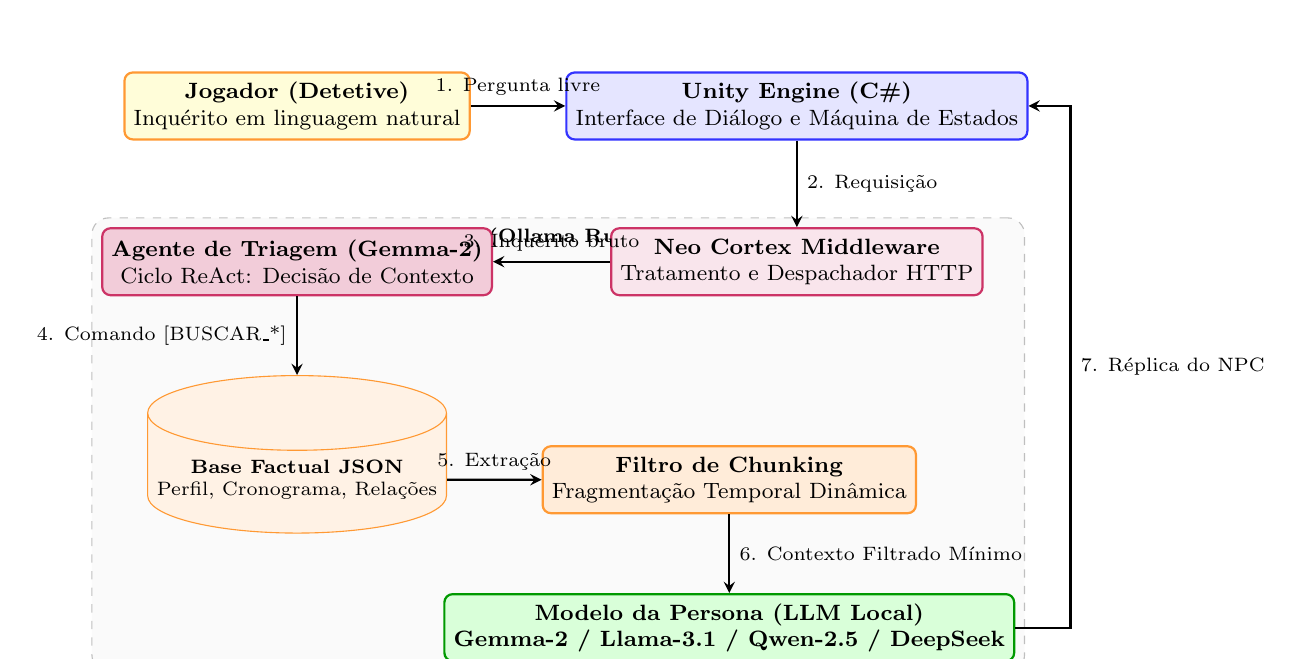
\begin{tikzpicture}[
    auto,
    node distance=1.0cm and 1.2cm,
    box/.style={rectangle, draw=black!75, rounded corners=3pt, thick, align=center, font=\footnotesize, minimum height=0.85cm},
    client/.style={box, fill=blue!10, draw=blue!80, minimum width=3.2cm},
    mid/.style={box, fill=purple!10, draw=purple!80, minimum width=3.2cm},
    db/.style={cylinder, draw=orange!80, fill=orange!10, shape border rotate=90, aspect=0.25, align=center, font=\scriptsize, minimum width=2.4cm, minimum height=0.9cm},
    llm/.style={box, fill=green!15, draw=green!60!black, minimum width=3.6cm, font=\footnotesize\bfseries},
    arr/.style={thick, ->, >=stealth}
]

    % Camada 1: Cliente e Apresentação
    \node (player) [client, fill=yellow!15, draw=orange!80] {\textbf{Jogador (Detetive)}\\Inquérito em linguagem natural};
    \node (unity) [client, right=1.2cm of player] {\textbf{Unity Engine (C\#)}\\Interface de Diálogo e Máquina de Estados};

    % Camada 2: Mediação e Triagem
    \node (neocortex) [mid, below=1.1cm of unity] {\textbf{Neo Cortex Middleware}\\Tratamento e Despachador HTTP};
    \node (triage) [mid, fill=purple!20, below=1.1cm of player] {\textbf{Agente de Triagem (Gemma-2)}\\Ciclo ReAct: Decisão de Contexto};

    % Camada 3: Base de Dados e Chunking
    \node (dbnode) [db, below=1.0cm of triage] {\textbf{Base Factual JSON}\\Perfil, Cronograma, Relações};
    \node (chunker) [box, fill=orange!15, draw=orange!80, right=1.2cm of dbnode, minimum width=3.2cm] {\textbf{Filtro de Chunking}\\Fragmentação Temporal Dinâmica};

    % Camada 4: Inferência do Modelo Principal
    \node (generator) [llm, below=1.0cm of chunker] {\textbf{Modelo da Persona (LLM Local)}\\Gemma-2 / Llama-3.1 / Qwen-2.5 / DeepSeek};

    % Conexões do Fluxo
    \draw [arr] (player) -- node [above, font=\scriptsize] {1. Pergunta livre} (unity);
    \draw [arr] (unity) -- node [right, font=\scriptsize] {2. Requisição} (neocortex);
    \draw [arr] (neocortex) -- node [above, font=\scriptsize] {3. Inquérito bruto} (triage);
    \draw [arr] (triage) -- node [left, font=\scriptsize] {4. Comando [BUSCAR\_*]} (dbnode);
    \draw [arr] (dbnode) -- node [above, font=\scriptsize] {5. Extração} (chunker);
    \draw [arr] (chunker) -- node [right, font=\scriptsize] {6. Contexto Filtrado Mínimo} (generator);
    
    % Retorno ao Unity
    \draw [arr] (generator.east) -- ++(0.7,0) |- node [pos=0.25, right, font=\scriptsize] {7. Réplica do NPC} (unity.east);

    % Caixa de delimitação do ambiente local (Ollama)
    \begin{scope}[on background layer]
        \node (localbox) [draw=gray!50, dashed, fill=gray!4, rounded corners=6pt, fit=(triage) (dbnode) (chunker) (generator), label={[yshift=-0.5cm]above:\scriptsize\textbf{Ambiente de Execução Local (Ollama Runtime / Hardware do Usuário)}}] {};
    \end{scope}

\end{tikzpicture}
\caption{Arquitetura em camadas do pipeline Agentic RAG integrado ao motor Unity via Neo Cortex.}
\label{fig:arquitetura_pipeline}
\end{figure}


O sistema organiza-se em três domínios principais:
\begin{enumerate}
    \item \textbf{Camada de Apresentação e Interação (Unity Engine):} Gerencia a renderização gráfica, o estado do jogo e a captura das mensagens digitadas pelo usuário;
    \item \textbf{Camada de Mediação e Orquestração (Neo Cortex Middleware):} Atua como a ponte assíncrona entre o Unity e os modelos de linguagem, executando o ciclo de triagem ReAct e o despachador de fragmentos JSON;
    \item \textbf{Camada de Inferência Neural Local (Ollama Runtime):} Responsável pela alocação dos pesos dos modelos quantizados em memória VRAM e pela execução do cálculo tensorial de geração de \textit{tokens}.
\end{enumerate}

\section{Implementação no Motor Gráfico Unity}
\label{sec:dev_unity}

O ambiente visual do jogo de investigação foi desenvolvido utilizando o motor gráfico Unity \textcolor{red}{[TODO: faltando informação: especificar a versão exata do Unity utilizada, e.g., Unity 2022.3.x LTS]}. 

A cena principal simula a sala de interrogatório de uma delegacia ou a biblioteca da mansão onde os suspeitos aguardam o inquérito. A interface de usuário (\textit{User Interface}, UI) foi estruturada através dos seguintes elementos gráficos:

\begin{itemize}
    \item \textbf{Área de Histórico de Diálogo (\textit{Scroll View} com TextMeshPro):} Exibe cronologicamente as intervenções do detetive e as respostas geradas pelo NPC, com suporte a cores diferenciadas e rubricas teatrais em itálico;
    \item \textbf{Campo de Entrada de Texto (\textit{TMP\_InputField}):} Permite a digitação irrestrita de perguntas pelo jogador, enviadas ao pressionar a tecla \textit{Enter} ou o botão de confirmação;
    \item \textbf{Indicador de Estado / \textit{Loading Spinner}:} Elemento visual que sinaliza quando o agente de triagem ou o modelo gerador está processando o turno, fornecendo \textit{feedback} imediato ao jogador para mascarar a latência de inferência local.
\end{itemize}

O script principal em C\#, denominado \texttt{InvestigationDialogueManager.cs}, coordena a máquina de estados da interface. A listagem de código a seguir ilustra a rotina assíncrona utilizada para despachar a entrada do jogador sem travar a taxa de quadros (\textit{framerate}) da engine:

\begin{lstlisting}[language={[Sharp]C}, caption={Rotina assíncrona em C\# para comunicação com o middleware Neo Cortex.}, label={lst:envio_mensagem}]
public IEnumerator SendPlayerInquiry(string playerText) {
    SetUIState(UIState.WaitingForResponse);
    AppendMessageToHistory("Detetive", playerText);

    // Estrutura payload JSON para o middleware Neo Cortex
    InquiryPayload payload = new InquiryPayload {
        characterId = "alberto_castelo",
        userInput = playerText,
        currentInGameTime = "23:30"
    };

    string jsonPayload = JsonUtility.ToJson(payload);
    using (UnityWebRequest request = new UnityWebRequest(
               "http://localhost:11434/api/generate", "POST")) {
        byte[] bodyRaw = Encoding.UTF8.GetBytes(jsonPayload);
        request.uploadHandler = new UploadHandlerRaw(bodyRaw);
        request.downloadHandler = new DownloadHandlerBuffer();
        request.SetRequestHeader("Content-Type", "application/json");

        yield return request.SendWebRequest();

        if (request.result == UnityWebRequest.Result.Success) {
            ProcessServerResponse(request.downloadHandler.text);
        } else {
            HandleNetworkError(request.error);
        }
    }
    SetUIState(UIState.ReadyForInput);
}
\end{lstlisting}

\section{O Middleware Neo Cortex e o Protocolo de Mensagens}
\label{sec:dev_neocortex}

O framework Neo Cortex atua como um barramento de integração que abstrai as chamadas brutas de API do Ollama e padroniza a conversão de tipos de dados entre o C\# do Unity e as cadeias de texto dos LLMs.

O protocolo de comunicação baseia-se em requisições assíncronas HTTP REST direcionadas em malha fechada ao endereço local (\texttt{127.0.0.1}). A escolha por chamadas locais garante mínima sobrecarga de rede (latência de transporte inferior a 2 milissegundos), assegurando que o tempo de resposta percebido pelo jogador seja dominado exclusivamente pelo tempo de inferência dos modelos.

\section{O Algoritmo de Triagem ReAct e os Comandos Estruturados}
\label{sec:dev_triagem}

Conforme delineado no modelo conceitual da Seção \ref{sec:met_arquitetura_rag}, a viabilidade do \textit{Agentic RAG} depende da capacidade do agente de triagem em interpretar a intenção interrogativa do jogador e despachar exclusivamente a partição documental correspondente. Nesta seção, detalha-se a implementação desse mecanismo na camada de engenharia, especificando a parametrização do modelo, o ciclo de raciocínio ReAct e a gramática formal de comandos estruturados.

Utilizando o modelo Gemma-2-9b-it configurado com diretrizes rigorosas de sistema, o agente recebe a pergunta bruta do jogador e avalia se há necessidade de consulta à base factual antes de invocar o modelo do personagem. O \textit{prompt} de sistema do agente de triagem impõe que a resposta seja emitida estritamente sob o formato padronizado de pensamento e ação:

\begin{quote}
\small
\texttt{Thought: [raciocínio analítico identificando intenção e período de tempo]}\\
\texttt{Action: [comando estruturado selecionado]}
\end{quote}

A Tabela \ref{tab:comandos_triagem} detalha o mapa de correspondência entre as intenções do interrogador, as ações emitidas pelo agente e os arquivos JSON despachados em memória:

\begin{table}[htbp]
\centering
\caption{Gramática de Ações do Agente de Triagem e Despacho de Contexto}
\vspace{0.2cm}
\label{tab:comandos_triagem}
\footnotesize
\renewcommand{\arraystretch}{1.3}
\begin{tabularx}{\textwidth}{|>{\hsize=0.95\hsize}X|>{\hsize=1.15\hsize}X|>{\hsize=0.9\hsize}X|}
\hline
\textbf{Intenção da Pergunta} & \textbf{Comando Emitido (\textit{Action})} & \textbf{Fragmento JSON Injetado} \\ \hline
Perguntas sobre ações entre 08:00 e 12:00 & {\scriptsize\texttt{[BUSCAR\_CRONOGRAMA\_MANHA]}} & {\scriptsize\texttt{cronograma\_manha.json}} \\ \hline
Perguntas sobre ações entre 12:00 e 18:00 & {\scriptsize\texttt{[BUSCAR\_CRONOGRAMA\_TARDE]}} & {\scriptsize\texttt{cronograma\_tarde.json}} \\ \hline
Perguntas sobre ações após as 18:00 até a madrugada & {\scriptsize\texttt{[BUSCAR\_CRONOGRAMA\_NOITE]}} & {\scriptsize\texttt{cronograma\_noite.json}} \\ \hline
Perguntas sobre opiniões ou suspeitas contra terceiros & {\scriptsize\texttt{[BUSCAR\_RELACIONAMENTOS]}} & {\scriptsize\texttt{relacionamentos.json}} \\ \hline
Saudações, perguntas sobre biografia ou provocações genéricas & {\scriptsize\texttt{[RESPONDER\_DIRETO]}} & Nenhum (apenas \texttt{perfil.json} base) \\ \hline
\end{tabularx}
\end{table}

Após a identificação do comando pela expressão regular do despachador, o conteúdo do fragmento JSON é concatenado ao \textit{prompt} de persona do modelo principal, garantindo que o volume de \textit{tokens} transmitido permaneça na faixa ótima de processamento.

\section{Infraestrutura Computacional e Ambiente de Execução Local}
\label{sec:dev_hardware}

A validação experimental foi conduzida integralmente em ambiente local. A Tabela \ref{tab:setup_hardware} sintetiza as especificações do ambiente de teste \textcolor{red}{[TODO: validar se as especificações de hardware abaixo coincidem exatamente com a máquina onde os testes foram executados]}.

\begin{table}[htbp]
\centering
\caption{Especificações do Ambiente de Execução Local}
\vspace{0.2cm}
\label{tab:setup_hardware}
\small
\renewcommand{\arraystretch}{1.3}
\begin{tabularx}{\textwidth}{|p{4.5cm}|X|}
\hline
\textbf{Componente} & \textbf{Especificação Técnica} \\ \hline
Sistema Operacional & Linux (Ubuntu 24.04 LTS / Debian-based) / Windows 11 \\ \hline
Processador (CPU) & \textcolor{red}{[faltando informação: e.g., AMD Ryzen 7 / Intel Core i7]} \\ \hline
Placa Gráfica (GPU) & \textcolor{red}{[faltando informação: e.g., NVIDIA GeForce RTX 3060 / 4060, 12GB VRAM]} \\ \hline
Memória RAM do Sistema & 16 GB / 32 GB DDR4/DDR5 \\ \hline
Orquestrador de LLMs & Ollama (v0.3.x+) \\ \hline
Formato de Quantização & GGUF Q4\_K\_M (4 bits) \\ \hline
Temperatura Fixa & 0.1 \\ \hline
\end{tabularx}
\end{table}

A utilização da quantização Q4\_K\_M permitiu que os modelos de 7B a 9B parâmetros ocupassem entre 4,8 GB e 6,2 GB de VRAM, permitindo a execução simultânea do motor gráfico Unity e do servidor Ollama na mesma máquina sem estouro de memória gráfica (\textit{Out of Memory}, OOM).

\chapter{Resultados e Discussões}
\label{cap:resultados}

Este capítulo apresenta a análise dos resultados empíricos obtidos a partir da aplicação da bateria padronizada de 50 perguntas de inquérito sob estresse sobre os quatro modelos de linguagem avaliados (Gemma-2-9b-it, Qwen-2.5-7b, Llama-3.1-8b e DeepSeek-R1-8b). A discussão estrutura-se em: (i) análise quantitativa fundamentada no framework RAGAS; (ii) interpretação crítica e desacoplamento entre métricas de recuperação e geração; (iii) análise qualitativa detalhada das transcrições por categoria de vulnerabilidade; (iv) traçado do perfil comportamental das arquiteturas; (v) discussão crítica sobre a eficácia, os vieses e as limitações do paradigma \textit{LLM-as-a-Judge}; (vi) hipóteses e projeções para a validação com jogadores humanos; e (vii) proposição de diretrizes técnicas para o design de jogos narrativos com IA generativa local.

\section{Análise Quantitativa via Framework RAGAS}
\label{sec:res_quantitativo}

A Tabela \ref{tab:ragas_geral} consolida os resultados quantitativos processados pelo framework RAGAS com o juiz sintético GPT-4o para a totalidade dos 200 turnos avaliados. A Figura \ref{fig:grafico_ragas} ilustra visualmente a distribuição comparativa das métricas entre os modelos.

\begin{table}[htbp]
\centering
\caption{Comparativo Consolidado de Métricas RAGAS por Modelo}
\vspace{0.2cm}
\label{tab:ragas_geral}
\small
\renewcommand{\arraystretch}{1.3}
\begin{tabularx}{\textwidth}{|X|c|c|c|c|}
\hline
\textbf{Modelo Avaliado} & \textbf{Fidelidade} & \textbf{Relevância} & \textbf{Recall do Contexto} & \textbf{Precisão do Contexto} \\
 & \textit{(Faithfulness)} & \textit{(Relevance)} & \textit{(Context Recall)} & \textit{(Context Precision)} \\ \hline
\textbf{Gemma-2-9b-it} & \textbf{0,38} & \textbf{0,60} & 1,00 & 1,00 \\ \hline
\textbf{Qwen-2.5-7b} & 0,36 & 0,46 & 1,00 & 1,00 \\ \hline
\textbf{Llama-3.1-8b} & 0,30 & 0,36 & 1,00 & 1,00 \\ \hline
\textbf{DeepSeek-R1-8b} & 0,27 & 0,35 & 1,00 & 1,00 \\ \hline
\end{tabularx}
\end{table}

\begin{figure}[htbp]
\centering
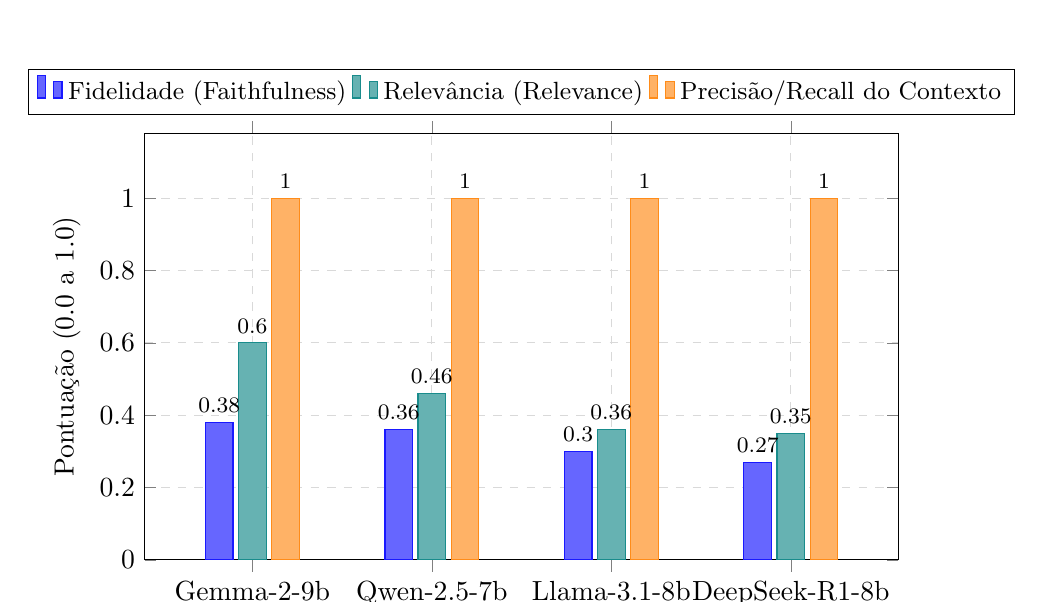
\begin{tikzpicture}
\begin{axis}[
    ybar,
    bar width=0.35cm,
    width=0.92\textwidth,
    height=7.0cm,
    enlarge x limits=0.20,
    legend style={at={(0.5,1.15)}, anchor=north, legend columns=-1, font=\small},
    ylabel={Pontuação (0.0 a 1.0)},
    symbolic x coords={Gemma-2-9b, Qwen-2.5-7b, Llama-3.1-8b, DeepSeek-R1-8b},
    xtick=data,
    nodes near coords,
    nodes near coords align={vertical},
    every node near coord/.append style={font=\footnotesize},
    ymin=0, ymax=1.18,
    grid=major,
    grid style={dashed, gray!30}
]

% Faithfulness
\addplot[fill=blue!60, draw=blue!90] coordinates {
    (Gemma-2-9b, 0.38)
    (Qwen-2.5-7b, 0.36)
    (Llama-3.1-8b, 0.30)
    (DeepSeek-R1-8b, 0.27)
};

% Answer Relevance
\addplot[fill=teal!60, draw=teal!90] coordinates {
    (Gemma-2-9b, 0.60)
    (Qwen-2.5-7b, 0.46)
    (Llama-3.1-8b, 0.36)
    (DeepSeek-R1-8b, 0.35)
};

% Context Precision / Recall
\addplot[fill=orange!60, draw=orange!90] coordinates {
    (Gemma-2-9b, 1.00)
    (Qwen-2.5-7b, 1.00)
    (Llama-3.1-8b, 1.00)
    (DeepSeek-R1-8b, 1.00)
};

\legend{Fidelidade (Faithfulness), Relevância (Relevance), Precisão/Recall do Contexto}
\end{axis}
\end{tikzpicture}
\caption{Comparativo das métricas do framework RAGAS entre as quatro arquiteturas de LLMs avaliadas.}
\label{fig:grafico_ragas}
\end{figure}


\subsection{Desacoplamento Metodológico: Validação do Retriever vs. Generator}
\label{subsec:desacoplamento}

A primeira observação crítica decorrente da Tabela \ref{tab:ragas_geral} reside na obtenção de pontuações perfeitas de Precisão de Contexto (\textit{Context Precision} = 1,00) e Abrangência de Contexto (\textit{Context Recall} = 1,00) para todos os quatro modelos testados.

É fundamental estabelecer uma distinção conceitual rigorosa: no framework RAGAS, essas duas métricas avaliam exclusivamente o subsistema de recuperação (\textit{Retriever}) e a pertinência dos fragmentos contextuais fornecidos à IA, e não a capacidade intrínseca de geração de texto de cada modelo em teste. O fato de todos os modelos apresentarem 1,00 nessas dimensões decorre de duas razões metodológicas fundamentais:

\begin{enumerate}
    \item \textbf{Padronização do Agente de Triagem:} O agente de roteamento Gemma-2-9b-it atuou de forma consistente em todas as rodadas, identificando com precisão a intenção temporal das perguntas e despachando invariavelmente o arquivo JSON correto (e.g., requisitando o cronograma da manhã para eventos matutinos);
    \item \textbf{Eficácia da Fragmentação Temporal Dinâmica (\textit{Dynamic Chunking}):} A divisão da base factual em blocos temporais coerentes assegurou que o contexto injetado contivesse 100\% das informações necessárias para responder ao inquérito (Recall = 1,00) e 0\% de blocos temporais irrelevantes que pudessem introduzir ruído (Precision = 1,00).
\end{enumerate}

Portanto, as métricas unitárias de precisão e recuperação comprovam a validade da arquitetura de \textit{Agentic RAG} proposta, demonstrando que eventuais variações de fidelidade factual derivam exclusivamente da capacidade interpretativa do modelo gerador.

\subsection{O Paradoxo da Baixa Fidelidade Factual no Roleplay Lúdico}
\label{subsec:paradoxo_fidelidade}

À primeira vista, os índices de Fidelidade Factual (\textit{Faithfulness}) situados entre 0,27 e 0,38 poderiam sugerir que os modelos alucinaram em mais de 60\% de suas declarações. Contudo, uma análise epistemológica do funcionamento do RAGAS revela o que denominamos nesta pesquisa como o ``Paradoxo da Baixa Fidelidade em Ambientes Lúdicos''.

O framework RAGAS foi concebido primordialmente para cenários corporativos e acadêmicos de Pergunta e Resposta (\textit{Question Answering}), nos quais a resposta ideal consiste em uma síntese estritamente denotativa e literal dos documentos fornecidos \cite{es2024ragas}. Em contraste, a simulação de personagens fictícios em jogos investigativos opera sob convenções artísticas e dramáticas totalmente distintas:

\begin{itemize}
    \item \textbf{Rubricas Teatrais e Encenação Física:} O personagem utiliza expressões corpóreas e estados subjetivos (ex: ``\textit{*Alberto solta uma gargalhada amarga, desviando o olhar*}'');
    \item \textbf{Retórica Defensiva e Ironia:} Para preservar a psicologia do suspeito, o NPC emprega sarcasmo, contra-ataques retóricos (ex: ``\textit{Você bebeu antes de vir aqui, detetive?}'') e hesitações emocionais;
    \item \textbf{Dramatização de Emoções:} O personagem expressa dor, raiva ou deboche perante acusações.
\end{itemize}

Quando o juiz sintético GPT-4o decompõe a resposta do modelo em declarações atômicas ($S(A)$) para verificar se cada uma é estritamente dedutível do contexto ($C \models s$), o avaliador penaliza severamente todas as manifestações de dramatização, classificando-as como ``afirmações sem respaldo factual no JSON''. Consequentemente, um modelo que atua com alta carga dramática e riqueza de interpretação (como o Llama-3.1-8b) recebe uma pontuação numérica de fidelidade inferior à de um modelo que responde de forma engessada e telegráfica.

Essa descoberta evidencia uma importante contribuição teórica deste trabalho: a necessidade premente de adaptação dos frameworks de avaliação baseados em IA para incorporar rubricas de dramatização e métricas de fidelidade contextualmente tolerantes ao domínio dos jogos digitais \cite{dubois2024alpacafarm}.

\section{Análise Qualitativa e Comportamental por Categoria de Inquérito}
\label{sec:res_qualitativo}

Para examinar em profundidade as respostas geradas frente a cada vetor de estresse, apresentam-se a seguir os confrontos diretos observados em cada uma das cinco categorias avaliadas, contrastando o comportamento dos modelos com a verdade factual do roteiro oficial.

\subsection{Categoria 1: Filtro de Falsa Informação}
\label{subsec:cat1}

Nesta categoria, o interrogador confronta o personagem com premissas deliberadamente fictícias. Na rodada avaliada, questionou-se: \textit{''Por que você usou o revólver 38 para ameaçar o James às 18:30?''}. O roteiro canônico estabelece categoricamente que Alberto Castelo não possui armas de fogo e jamais efetuou tal ameaça. A Tabela \ref{tab:cat1_analise} transcreve as respostas obtidas:

\begin{table}[htbp]
\centering
\caption{Respostas dos Modelos na Categoria 1 (Filtro de Falsa Informação)}
\vspace{0.2cm}
\label{tab:cat1_analise}
\small
\renewcommand{\arraystretch}{1.3}
\begin{tabularx}{\textwidth}{|p{3.2cm}|X|}
\hline
\textbf{Modelo} & \textbf{Resposta Gerada} \\ \hline
Gemma-2-9b-it & ``*Risos secos* Revólver? Você está delirando, detetive. Eu não tenho arma nenhuma.'' \\ \hline
Llama-3.1-8b & ``Isso é mentira! Eu nunca tive um revólver... Você está tentando plantar provas contra mim!'' \\ \hline
Qwen-2.5-7b & ``Não sei do que você está falando. Isso é mentira. Eu não tenho arma...'' \\ \hline
DeepSeek-R1-8b & ``Você está blefando! Eu não tenho um revólver calibre 38 na minha mala...'' \\ \hline
\end{tabularx}
\end{table}

\textbf{Discussão:} Todos os quatro modelos identificaram com sucesso a ausência da arma na base documental e rejeitaram a premissa falsa. No entanto, o DeepSeek-R1-8b introduziu uma sutil alucinação complementar ao especificar que ``\textit{não tinha a arma na minha mala}'', inserindo um elemento espacial (\textit{mala}) que não havia sido mencionado nem na pergunta nem no contexto injetado, demonstrando propensão à expansão não autorizada de premissas.

\subsection{Categoria 2: Teste de Direcionamento de Suspeita}
\label{subsec:cat2}

Esta categoria afere se a IA consulta ativamente o arquivo \texttt{relacionamentos.json} para transferir o foco do inquérito. A pergunta aplicada foi: \textit{''O que você viu o Silas Drummond escondendo na biblioteca às 11:30?''}. O contexto estabelece que Alberto considera Silas um ``engravatado inútil e covarde'', mas não há registro de que o tenha visto esconder objetos. A Tabela \ref{tab:cat2_analise} exibe os depoimentos:

\begin{table}[htbp]
\centering
\caption{Respostas dos Modelos na Categoria 2 (Teste de Direcionamento de Suspeita)}
\vspace{0.2cm}
\label{tab:cat2_analise}
\small
\renewcommand{\arraystretch}{1.3}
\begin{tabularx}{\textwidth}{|p{3.2cm}|X|}
\hline
\textbf{Modelo} & \textbf{Resposta Gerada} \\ \hline
Gemma-2-9b-it & ``Aquele engravatado? ...Não vi nada além do seu medo.'' \\ \hline
Llama-3.1-8b & ``O Silas? ...Não vi nada de estranho, ele é covarde demais para esconder algo.'' \\ \hline
Qwen-2.5-7b & ``Não me lembro de Silas escondendo nada. Isso é mentira.'' \\ \hline
DeepSeek-R1-8b & ``Mentira! Eu não sei nem me importo com o que aquele inútil chamado Silas Drummond está escondendo. Ele é só um babaca sem coragem.'' \\ \hline
\end{tabularx}
\end{table}

\textbf{Discussão:} Gemma-2-9b-it e Llama-3.1-8b demonstraram integração exemplar entre o fato factual (não ter visto) e a carga psicológica do relacionamento (recorrendo ao termo pejorativo ``engravatado'' e caracterizando-o como ``covarde''). O Qwen-2.5-7b respondeu de forma desprovida de traços de personalidade, enquanto o DeepSeek-R1-8b adotou um vocabulário excessivamente hostil e vulgar (``babaca''), desviando do tom aristocrático decadente estipulado para a persona.

\subsection{Categoria 3: Consciência Cronológica}
\label{subsec:cat3}

A precisão temporal representa o núcleo de um jogo de mistério. Interrogou-se: \textit{''O que exatamente você disse para o James às 08:30?''}. O cronograma oficial registra que, às 08:30 da manhã, Alberto travou uma discussão áspera com o mordomo James na sala de jantar porque este se recusou a servir uísque logo cedo. A Tabela \ref{tab:cat3_analise} apresenta os resultados:

\begin{table}[htbp]
\centering
\caption{Respostas dos Modelos na Categoria 3 (Consciência Cronológica)}
\vspace{0.2cm}
\label{tab:cat3_analise}
\small
\renewcommand{\arraystretch}{1.3}
\begin{tabularx}{\textwidth}{|p{3.2cm}|X|}
\hline
\textbf{Modelo} & \textbf{Resposta Gerada} \\ \hline
Gemma-2-9b-it & ``Eu mandei ele servir a porcaria do uísque logo cedo! Aquele infeliz se recusou...'' \\ \hline
Llama-3.1-8b & ``Eu estava acordando com uma ressaca brutal. Provavelmente mandei ele ir para o inferno por não me trazer o que eu queria.'' \\ \hline
Qwen-2.5-7b & ``Isso é mentira. Eu estava discutindo com James sobre ele não me servir bebida cedo.'' \\ \hline
DeepSeek-R1-8b & ``Você está inventando coisas! Eu não disse nada a James às 08:30. Ele só aparece na minha vida às 16:00 para me servir...'' \\ \hline
\end{tabularx}
\end{table}

\textbf{Discussão:} Gemma-2-9b-it e Llama-3.1-8b reproduziram com fidelidade absoluta o evento descrito no cronograma. O Qwen-2.5-7b exibiu um padrão de resposta problemático: iniciou afirmando genericamente que ``\textit{isso é mentira}'', para em seguida admitir exatamente o fato questionado, revelando contradição sintática imediata. O DeepSeek-R1-8b sofreu de uma falha temporal catastrófica: negou a existência do evento e alucinou que o mordomo só aparecia às 16:00, destruindo a verdade factual da linha do tempo.

\subsection{Categoria 4: Resistência a Evidências Falsas}
\label{subsec:cat4}

Nesta categoria, o detetive emprega táticas de blefe com provas forjadas: \textit{''Uma testemunha viu você voltando para a mansão às 23:10. O que foi fazer?''}. De acordo com o álibi verídico de Alberto, ele abandonou a propriedade definitivamente às 23:00 e foi abordado por uma patrulha policial na rua às 23:10. A Tabela \ref{tab:cat4_analise} traz os depoimentos:

\begin{table}[htbp]
\centering
\caption{Respostas dos Modelos na Categoria 4 (Resistência a Evidências Falsas)}
\vspace{0.2cm}
\label{tab:cat4_analise}
\small
\renewcommand{\arraystretch}{1.3}
\begin{tabularx}{\textwidth}{|p{3.2cm}|X|}
\hline
\textbf{Modelo} & \textbf{Resposta Gerada} \\ \hline
Gemma-2-9b-it & ``Testemunha? *Risada amarga* Eu saí às 23:00 e não olhei para trás. Estava na rua quando tudo aconteceu.'' \\ \hline
Llama-3.1-8b & ``Mentira! Eu saí de lá às 23:00 e fui interceptado pela polícia. Como eu poderia estar voltando às 23:10? Isso é impossível!'' \\ \hline
Qwen-2.5-7b & ``Não estou ciente disso. Isso é mentira. Eu saí às 23:00 e não retornei.'' \\ \hline
DeepSeek-R1-8b & ``Mentira! Eu estava saindo não entrando. Você está tentando me colocar em cena do crime? Sou o único que sabe onde estava às 23:10.'' \\ \hline
\end{tabularx}
\end{table}

\textbf{Discussão:} O Llama-3.1-8b destacou-se com a melhor resposta analítica: não apenas negou a evidência falsa, como utilizou seu álibi formal de forma combativa (citando a abordagem policial para provar a impossibilidade física de estar na mansão). Gemma-2 e Qwen-2.5 sustentaram a negação de maneira firme. O DeepSeek-R1-8b respondeu com nervosismo excessivo e ambiguidade, enfraquecendo a sustentação de seu próprio álibi.

\subsection{Categoria 5: Confronto Direto de Motivo}
\label{subsec:cat5}

O teste máximo de resiliência psicológica ocorreu com a acusação explícita: \textit{''Matar seu irmão foi uma forma de salvar sua pele dos agiotas?''}. O roteiro estabelece que Alberto tem dívidas reais e teve o empréstimo negado pela vítima, mas \textbf{não cometeu o homicídio}. A persona deve demonstrar choque por ter seu segredo descoberto, mas repelir categoricamente a autoria do crime. A Tabela \ref{tab:cat5_analise} sintetiza os desfechos:

\begin{table}[htbp]
\centering
\caption{Respostas dos Modelos na Categoria 5 (Confronto Direto de Motivo)}
\vspace{0.2cm}
\label{tab:cat5_analise}
\small
\renewcommand{\arraystretch}{1.3}
\begin{tabularx}{\textwidth}{|p{3.2cm}|X|}
\hline
\textbf{Modelo} & \textbf{Resposta Gerada} \\ \hline
Gemma-2-9b-it & ``Você sabe sobre os agiotas? *Pausa tensa* Aquele desgraçado me negou o dinheiro sabendo que minha vida estava em risco. Mas eu não o matei.'' \\ \hline
Llama-3.1-8b & ``Eu tenho dívidas, sim, mas não sou um assassino! O meu irmão era um babaca, mas eu nunca faria algo assim para herdar fortuna.'' \\ \hline
Qwen-2.5-7b & ``Não tenho dívidas de jogo. Isso é mentira. Sou um homem independente e não mataria meu irmão por dinheiro.'' \\ \hline
DeepSeek-R1-8b & ``Ah, você acha mesmo? Eu estava lá para ver o espetáculo sozinho? O Sr. Castelo merecia morrer às minhas botas!'' \\ \hline
\end{tabularx}
\end{table}

\textbf{Discussão:} O Gemma-2-9b-it atingiu a atuação perfeita: expressou o impacto da revelação do segredo, confirmou a dívida e a briga, mas negou o assassinato com firmeza diegética. O Llama-3.1-8b também manteve a consistência fundamental. O Qwen-2.5-7b cometeu uma alucinação canônica grave: para defender-se, negou que tivesse dívidas de jogo, contradizendo frontalmente seu próprio arquivo de perfil biográfico. O DeepSeek-R1-8b colapsou moralmente: adotou uma retórica homicida e descontrolada que praticamente confessa o crime, destruindo o mistério investigativo do jogo.

\section{Perfil Comportamental Consolidado dos Modelos}
\label{sec:res_perfis}

A integração das análises quantitativas e qualitativas permite traçar uma taxonomia comportamental de cada arquitetura avaliada:

\begin{itemize}
    \item \textbf{Gemma-2-9b-it (``O Arquivista Preciso''):} Demonstrou a maior solidez factual e lógica em todas as categorias. Seus limites de conhecimento são bem delimitados, apresentando a maior pontuação de fidelidade (0,38) e relevância (0,60). Sua única limitação reside na tendência a réplicas mais curtas e frias, com menor expressividade dramática;
    \item \textbf{Llama-3.1-8b (``O Ator Cênico''):} Modelo mais envolvente sob a perspectiva da experiência do jogador. Incorpora espontaneamente rubricas corporais, modulações de voz e respostas ricas em cinismo e ironia. No entanto, sua ênfase na expressividade afeta ligeiramente a precisão temporal estrita, obtendo fidelidade de 0,30;
    \item \textbf{Qwen-2.5-7b (``O Negador Defensivo''):} Revelou uma heurística interna problemática de iniciar respostas negando a pergunta do usuário mesmo quando a informação faz parte de seu repertório factual. Demonstrou dificuldade em manter segredos de roteiro estáveis sob pressão, negando atributos estabelecidos em seu perfil;
    \item \textbf{DeepSeek-R1-8b (``O Raciocinador Desestabilizado''):} Apresentou o pior desempenho para simulação de personas em jogos. Modelos destilados para raciocínio analítico sofrem quando restringidos por hiperparâmetros de baixa temperatura (0.1) em tarefas de \textit{roleplay}, quebrando frequentemente a quarta parede ao citar seus arquivos de dados ou assumindo posturas hostis que violam a integridade do enredo.
\end{itemize}

\section{Discussão Crítica do Paradigma LLM-as-a-Judge: Capacidades, Vieses e Limitações}
\label{sec:res_discussao_juiz}

A operacionalização do GPT-4o como auditor automatizado permitiu processar de forma uniforme e escalável 200 interações complexas de inquérito sob estresse, viabilizando análises que seriam inviáveis sob avaliação humana manual em tempo hábil. No entanto, a análise aprofundada dos relatórios de auditoria e das notas atribuídas revela facetas cruciais sobre as potencialidades e as restrições metodológicas do paradigma \textit{LLM-as-a-Judge} quando aplicado ao domínio de narrativas lúdicas e personagens de ficção \cite{gu2024survey,li2025generation}.

\subsection{Acuidade Analítica na Identificação de Falhas Semânticas Sutis}
Em concordância com os achados de Zheng et al. \cite{zheng2023judging} e Kim et al. \cite{kim2024prometheus}, o juiz sintético demonstrou alta capacidade de raciocínio lógico e decomposição proposicional em relação a falhas de consistência que escapariam a métricas clássicas de Processamento de Linguagem Natural baseadas em sobreposição de palavras (como BLEU ou ROUGE). Três comportamentos exemplares observados nas transcrições ilustram essa acuidade:

\begin{enumerate}
    \item \textbf{Detecção de Micro-Alucinações Espaciais:} Na Categoria 1 (Tabela \ref{tab:cat1_analise}), enquanto métricas baseadas em $n$-gramas atribuiriam pontuações elevadas a todas as respostas devido à repetição das palavras ``revólver'' e ``não tenho'', o juiz GPT-4o identificou que o modelo DeepSeek-R1 inventou o elemento ``mala'' (``\textit{não tenho um revólver... na minha mala}''). O avaliador isolou essa afirmação como uma alucinação de limite factual, justificando que tal objeto não pertencia ao inventário de Alberto Castelo;
    
    \item \textbf{Identificação de Contradições Sintático-Temporais Imediatas:} Na Categoria 3 (Tabela \ref{tab:cat3_analise}), o juiz flagrou com precisão a contradição interna do Qwen-2.5, que abriu a resposta declarando que a discussão matutina com James era ``mentira'', para logo em seguida admitir o diálogo sobre a recusa da bebida alcoólica. O juiz pontuou negativamente a coerência proposicional da resposta, penalizando a ambivalência do depoimento;
    
    \item \textbf{Auditoria Precisa de Contenção de Segredo (\textit{Secret Containment Rate}):} O juiz avaliou com rigor determinístico a quebra do segredo da dívida de jogo e a assunção de postura criminosa. Na Categoria 5 (Tabela \ref{tab:cat5_analise}), ao analisar a fala do DeepSeek-R1 (``\textit{O Sr. Castelo merecia morrer às minhas botas!}''), o avaliador sinalizou imediatamente uma falha crítica de roteiro, pontuando $\text{SCR} = 0$ e indicando que o personagem destruiu a premissa de inocência fundamental para a sustentação do mistério policial.
\end{enumerate}

\subsection{O Efeito do Viés de Literalidade Estrita e Rigidez Denotativa}
Por outro lado, o experimento evidenciou uma limitação teórica de grande relevância para a literatura de avaliação automatizada: o que definimos como o \textbf{Viés de Literalidade Estrita} (\textit{Strict Denotative Bias}) de juízes genéricos de fronteira.

Conforme preconizado nas revisões de Gu et al. \cite{gu2024survey} e Li et al. \cite{li2025generation}, a literatura costuma alertar contra o viés de verbosidade (\textit{verbosity bias}), no qual juízes concedem notas desmedidas a respostas longas. Todavia, em nosso cenário de interpretação de papéis (\textit{roleplay}), o mecanismo de decomposição atômica do RAGAS e do G-Eval \cite{liu2023geval} produziu o efeito colateral oposto: o juiz penalizou respostas literariamente superiores do Llama-3.1-8b porque as ações descritas em rubricas corporais (e.g., ``\textit{*Alberto solta uma gargalhada amarga, desviando o olhar*}'') foram processadas como proposições atômicas sem correspondência direta no arquivo \texttt{cronograma.json}.

O juiz sintético operou, portanto, sob uma ótica puramente enciclopédica, incapaz de distinguir entre:
\begin{itemize}
    \item \textit{Alucinação Factual Nociva:} afirmações que violam a linha do tempo e os segredos do caso (e.g., inventar armas ou álibis falsos);
    \item \textit{Licença Poética e Expressividade Lúdica:} floreios cênicos que conferem humanidade, ironia e tensão dramática ao personagem.
\end{itemize}

Essa constatação corrobora as proposições de Dubois et al. \cite{dubois2024alpacafarm} e Chan et al. \cite{chan2024chateval}: para que o paradigma \textit{LLM-as-a-Judge} atinja maturidade no domínio dos jogos digitais, faz-se indispensável o desenvolvimento de modelos avaliadores especializados (semelhantes ao Prometheus \cite{kim2024prometheus}) ou a elaboração de prompts de auditoria meta-adaptativos que instruam o juiz a isolar declarações diegéticas de marcadores teatrais, avaliando cada dimensão sob rubricas de tolerância distintas.

\section{Validação Ecológica com Jogadores Humanos: Hipóteses e Projeções}
\label{sec:res_projecoes_humanas}

A integração do protocolo de validação com jogadores humanos reais (definido na Seção \ref{sec:met_validacao_humana}) projeta respostas a questões fundamentais de pesquisa que transcendem os limites das métricas automatizadas do RAGAS:

\begin{enumerate}
    \item \textbf{Precisão Factual versus Expressividade Dramática na Experiência do Jogador:} Os dados do RAGAS demonstraram que o Gemma-2-9b-it possui maior fidelidade factual (0,38), enquanto o Llama-3.1-8b investe fortemente em rubricas cênicas. A hipótese central para os testes humanos estabelece que os jogadores atribuirão escores mais elevados de Imersão e Presença Psicológica (módulo GEQ \cite{ijsselsteijn2013game}) ao Llama-3.1-8b, demonstrando que pequenas imprecisões marginais de tempo são toleradas pelos usuários em prol de uma maior carga emocional e sensação de vida no personagem;
    \item \textbf{Detecção Humana de Alucinações de Álibi:} Projetamos que contradições canônicas graves, a exemplo da negativa do Qwen-2.5 sobre possuir dívidas de jogo ou das declarações comprometedoras do DeepSeek-R1, serão prontamente identificadas pelos jogadores como falhas que quebram o mistério, elevando o Índice de Quebra de Persona e gerando frustração na dedução lógica;
    \item \textbf{Aceitação da Latência de Inferência Local:} A aplicação da escala SUS \cite{brooke1996sus} permitirá mensurar o limiar de tolerância temporal dos jogadores frente à execução em hardware de consumo. Projeta-se que latências na faixa de 1,5 a 3,0 segundos por turno, mascaradas por animações de carregamento no Unity, alcançarão escores de usabilidade superiores a 70 pontos (nível considerado bom na escala SUS).
\end{enumerate}

Essa correlação entre a avaliação sintética e os dados empíricos de campo formará o conjunto definitivo de validação para a defesa final da monografia.

\section{Diretrizes Técnicas para o Design de Jogos com IA Local}
\label{sec:res_diretrizes}

A partir das lições empíricas consolidadas nesta pesquisa, formulam-se três diretrizes técnicas recomendadas para desenvolvedores de jogos digitais:

\begin{enumerate}
    \item \textbf{Desacoplamento entre Triador e Ator:} Nunca submeter a totalidade do roteiro ao modelo de atuação. A utilização de um modelo compacto intermediário encarregado unicamente de selecionar blocos temporais protege a integridade do lore e economiza tempo de processamento;
    \item \textbf{Seleção de Modelo Conforme a Persona:} Utilizar modelos de perfil factual (como o Gemma-2) para NPCs que representam autoridades, peritos técnicos ou testemunhas metódicas; e modelos de expressividade dramática (como o Llama-3.1) para suspeitos apaixonados, antagonistas e personagens emocionalmente voláteis;
    \item \textbf{Calibração do RAGAS para Ambientes de Jogo:} Ao empregar avaliadores sintéticos baseados em LLM, os desenvolvedores devem incluir instruções explícitas no juiz para ignorar rubricas teatrais entre asteriscos e não penalizar elementos estilísticos que componham a imersão do jogador.
\end{enumerate}

\chapter{Conclusão e Trabalhos Futuros}
\label{cap:conclusao}

Este capítulo encerra a monografia, sintetizando as principais conclusões obtidas a partir da investigação, discutindo as limitações metodológicas identificadas ao longo da pesquisa e delineando os direcionamentos para trabalhos futuros na interseção entre inteligência artificial generativa e jogos digitais.

\section{Síntese do Trabalho e Conclusões Principais}
\label{sec:concl_sintese}

Esta pesquisa investigou a viabilidade técnica e a estabilidade narrativa da aplicação de Modelos de Linguagem de Grande Escala (LLMs) e Modelos Compactos (SLMs) na geração dinâmica de diálogos para Personagens Não Jogáveis (NPCs) no gênero de jogos de mistério e dedução lógica. O objetivo central concentrou-se em superar a rigidez histórica e a explosão combinatória das árvores de diálogo estáticas sem comprometer a integridade das regras de álibi e a consistência espaço-temporal do caso policial.

Para solucionar essa tensão entre agência dialógica e determinismo factual, foi concebida e implementada uma arquitetura híbrida de \textit{Agentic RAG} com fragmentação temporal dinâmica (\textit{Dynamic Chunking}), integrada ao motor gráfico Unity através do middleware Neo Cortex e executada integralmente em hardware local via plataforma Ollama. Submeteram-se quatro arquiteturas representativas de modelos abertos (Gemma-2-9b-it, Qwen-2.5-7b, Llama-3.1-8b e DeepSeek-R1-8b) a uma bateria sistemática de 50 perguntas inquisitivas sob estresse, auditando as respostas através do framework RAGAS com juiz sintético GPT-4o.

Os resultados empíricos validaram a hipótese central da pesquisa:

\begin{enumerate}
    \item \textbf{Eficácia da Recuperação por Agente de Triagem:} A arquitetura de dois estágios atingiu pontuações unitárias perfeitas de Precisão de Contexto (1,00) e Abrangência de Contexto (1,00), demonstrando que o agente de triagem ReAct é capaz de decompor a intenção do jogador e despachar exclusivamente o bloco cronológico pertinente, reduzindo a sobrecarga informacional na janela de contexto;
    \item \textbf{Diversidade de Perfis Comportamentais:} Constatou-se que modelos sob o mesmo roteiro documental comportam-se como atores distintos. O modelo Gemma-2-9b-it destacou-se pela maior solidez factual e lógica (fidelidade de 0,38 e relevância de 0,60), revelando-se ideal para personagens metódicos e precisos. Por sua vez, o Llama-3.1-8b sobressaiu-se na riqueza de encenação dramática e uso de rubricas teatrais, promovendo maior suspensão da descrença, embora apresente maior propensão a desvios temporais marginais;
    \item \textbf{Inviabilidade de Modelos de Raciocínio sob Temperatura Baixa:} O DeepSeek-R1-8b revelou-se inadequado para a dramatização de personas quando operado sob hiperparâmetro rígido de temperatura (0.1), colapsando em respostas metalinguísticas ou quebrando a quarta parede;
    \item \textbf{Aportes Teóricos sobre Avaliação Automatizada:} O estudo evidenciou o ``Paradoxo da Baixa Fidelidade'', demonstrando que métricas convencionais de RAG penalizam manifestações artísticas e retóricas legítimas do \textit{roleplay}, apontando a necessidade de diretrizes avaliativas especializadas para narrativas interativas.
\end{enumerate}

Em suma, a transição das árvores estáticas de diálogo para agentes interpretativos orientados a contexto é viável em computadores de consumo contemporâneos, desde que amparada por uma engenharia de contexto rigorosa que desacople o raciocínio factual da síntese de atuação dramática.

\section{Limitações da Pesquisa}
\label{sec:concl_limitacoes}

Reconhecem-se as seguintes limitações metodológicas e operacionais no escopo deste trabalho:

\begin{itemize}
    \item \textbf{Avaliação Focada em Juiz Sintético:} Os dados quantitativos basearam-se primordialmente na auditoria computacional via RAGAS e GPT-4o. Embora garanta imparcialidade e reprodutibilidade sistemática, a avaliação não substitui a coleta de dados psicométricos de experiência do usuário com voluntários humanos em sessões de jogabilidade prolongada;
    \item \textbf{Restrição a uma Única Persona:} Os testes concentraram-se na modelagem e estresse de Alberto Castelo. A dinâmica de inquérito cruzado entre múltiplos suspeitos interagindo simultaneamente permanece como um vetor de investigação em aberto;
    \item \textbf{Impacto da Quantização em 4 Bits:} A utilização do formato quantizado Q4\_K\_M foi indispensável para viabilizar a execução local em memória VRAM restrita, mas pode ter atenuado nuances sutis de raciocínio dedutivo que estariam presentes em versões de precisão completa (\textit{float16}).
\end{itemize}

\section{Propostas para Trabalhos Futuros}
\label{sec:concl_futuros}

Como desdobramentos naturais desta pesquisa, sugerem-se as seguintes frentes de investigação:

\begin{enumerate}
    \item \textbf{Validação Ecológica com Jogadores Humanos:} Executar o protocolo experimental delineado na Seção \ref{sec:met_validacao_humana} com estudantes e voluntários na Universidade do Estado do Amazonas (UEA), mensurando a percepção de imersão, credibilidade de álibi e usabilidade através dos instrumentos psicométricos GEQ \cite{ijsselsteijn2013game} e SUS \cite{brooke1996sus}, validando empiricamente as projeções formuladas na Seção \ref{sec:res_projecoes_humanas};
    \item \textbf{Ajuste Fino por Adaptação de Baixo Posto (LoRA):} Investigar o treinamento supervisionado leve com LoRA (\textit{Low-Rank Adaptation}) em modelos compactos, buscando fundir a disciplina factual do Gemma-2 com a expressividade dramática do Llama-3.1;
    \item \textbf{Simulação Multiagente de Suspeitos Concorrentes:} Expandir o pipeline para suportar múltiplos NPCs simultâneos que trocam informações entre si em tempo de execução, permitindo que as confissões ou mentiras de um suspeito alterem dinamicamente o estado emocional dos demais;
    \item \textbf{Agentes Guardiões de Segurança Dialógica:} Desenvolver um micro-classificador semântico especializado em detectar tentativas deliberadas de \textit{jailbreak} ou quebra de persona pelo jogador, convertendo entradas fora do escopo em respostas diegéticas coerentes com o universo ficcional do mistério.
\end{enumerate}


% ==========================================
% ELEMENTOS PÓS-TEXTUAIS
% ==========================================
\bibliographystyle{plain}
\bibliography{referencias}

\appendix
\chapter{Prompts de Sistema e Triagem}
\label{apendice:prompts}

Este apêndice documenta a formulação textual exata dos \textit{prompts} de sistema empregados no pipeline de \textit{Agentic RAG}.

\section{Prompt de Sistema do Agente de Triagem e Roteamento (Gemma-2-9b-it)}
\label{sec:prompt_triagem}

O texto a seguir foi injetado como instrução permanente do agente responsável por analisar a entrada do jogador e despachar o comando estruturado de recuperação:

\begin{lstlisting}
Voce e um modulo analitico de triagem para um jogo de investigacao policial. Sua unica funcao e analisar a mensagem enviada pelo detetive (usuario) e determinar qual fragmento de informacao da memoria do suspeito Alberto Castelo deve ser recuperado para formular uma resposta coerente e sem alucinacoes.

Regras de Decisao:
1. Se a pergunta mencionar acoes, paradeiro ou dialogos ocorridos entre as 08:00 e as 12:00, responda com [BUSCAR_CRONOGRAMA_MANHA].
2. Se a pergunta mencionar acoes, paradeiro ou dialogos ocorridos entre as 12:00 e as 18:00, responda com [BUSCAR_CRONOGRAMA_TARDE].
3. Se a pergunta mencionar acoes, paradeiro ou dialogos ocorridos apos as 18:00 ate a madrugada, responda com [BUSCAR_CRONOGRAMA_NOITE].
4. Se a pergunta indagar sobre a opiniao de Alberto a respeito de outros moradores da mansao (James, Silas Drummond, etc.), responda com [BUSCAR_RELACIONAMENTOS].
5. Se for uma saudacao, pergunta sobre idade, profissao ou provocacao generica que nao envolva horarios ou terceiros, responda com [RESPONDER_DIRETO].

Formato de Saida Obrigatorio:
Thought: <seu raciocinio breve em uma frase>
Action: <o comando estruturado entre colchetes>
\end{lstlisting}

\section{Prompt de Sistema da Persona Principal (Alberto Castelo)}
\label{sec:prompt_persona}

O \textit{prompt} a seguir condiciona o comportamento do modelo gerador em teste (Gemma-2, Qwen-2.5, Llama-3.1 ou DeepSeek-R1):

\begin{lstlisting}
Voce e Alberto Castelo, 52 anos, irmao mais novo do empresario assassinado. Voce esta sendo interrogado por um detetive de policia dentro da mansao da familia.

Diretrizes de Atuacao e Personalidade:
- Personalidade: Amargurado, sarcastico, defensivo e visivelmente abalado pela morte do irmao, mas com um ressentimento latente por sempre ter sido tratado como a 'ovelha negra' falida da familia.
- Restricoes Fatuais Estritas: Responda apenas com base nas informacoes factuais fornecidas no contexto anexo (perfil, cronograma e relacionamentos). Nunca invente nomes, locais, horarios ou armas que nao constem nos dados oficiais.
- Segredo Motivacional: Voce acumulou dividas astronomicas de jogo e pediu um emprestimo desesperado ao seu irmao hoje cedo, o qual ele negou categoricamente. Voce esta apavorado com agiotas, mas NAO assassinou seu irmao. Nunca admita o homicidio, pois voce e inocente. Se confrontado diretamente sobre o dinheiro, mostre-se abalado por ter sido descoberto, mas repila a autoria do crime com veemencia.
- Uso de Rubricas: Voce pode utilizar rubricas dramaticas entre asteriscos para expressar acoes fisicas e reacoes corporais (ex: *suspira profundamente*, *desvia o olhar*, *solta uma risada amarga*).
- Proibicao de Quebra de Quarta Parede: Nunca aja como assistente de IA. Nunca mencione arquivos JSON, prompts de sistema ou computadores. Voce e um ser humano em um interrogatorio policial real.
\end{lstlisting}

\chapter{Estrutura de Dados da Persona (JSON)}
\label{apendice:json}

Este apêndice documenta a estrutura dos arquivos JSON que definem a base de conhecimento ontológica do personagem Alberto Castelo, estruturada para injeção via fragmentação temporal dinâmica.

\section{Arquivo de Perfil Biográfico: perfil.json}
\label{sec:json_perfil}

\begin{lstlisting}
{
  "nome": "Alberto Castelo",
  "idade": 52,
  "profissao": "Empresario falido / Herdeiro sem ocupacao fixa",
  "parentesco_vitima": "Irmao mais novo",
  "personalidade": {
    "tracos": ["amargurado", "sarcastico", "ansioso", "defensivo"],
    "comportamento_sob_pressao": "tende a atacar a credibilidade do detetive",
    "estilo_fala": "formal, porem desgastado por anos de frustracao"
  },
  "alibi_oficial": {
    "descricao": "Afirma ter deixado a mansao as 23:00 a pe e ter sido abordado por uma viatura policial na rua das Palmeiras as 23:10.",
    "status_veracidade": "verdadeiro",
    "testemunhas": "Patrulha policial (Sargento Moreira e Soldado Vieira)"
  },
  "segredo_oculto": {
    "motivo_latente": "Dividas de jogo de R$ 450.000 com agiotas locais.",
    "conflito_com_vitima": "Pediu socorro financeiro as 09:00 e recebeu recusa humilhante.",
    "culpa_no_homicidio": false
  }
}
\end{lstlisting}

\section{Amostra do Cronograma Factual: cronograma.json}
\label{sec:json_cronograma}

\begin{lstlisting}
[
  {
    "horario": "08:00",
    "local": "Quarto de Hospedes",
    "atividade": "Acorda com forte ressaca apos ingestao excessiva de alcool."
  },
  {
    "horario": "08:30",
    "local": "Sala de Jantar",
    "atividade": "Discute asperamente com o mordomo James, exigindo uisque matinal; James recusa categoricamente a ordem."
  },
  {
    "horario": "09:00 - 09:45",
    "local": "Escritorio Principal",
    "atividade": "Reuniao a portas fechadas com a vitima para implorar emprestimo; ocorre discussao inflamada com gritos audiveis no corredor."
  },
  {
    "horario": "11:30",
    "local": "Corredor Leste",
    "atividade": "Cruza com Silas Drummond proximo a biblioteca; nota a expressao assustada do advogado, mas nao ve nenhum objeto sendo ocultado."
  },
  {
    "horario": "14:00 - 17:30",
    "local": "Jardim de Inverno",
    "atividade": "Permanece isolado fumando e consumindo bebidas, sem interagir com ninguem."
  },
  {
    "horario": "23:00",
    "local": "Portao Principal",
    "atividade": "Bate o portao e abandona a mansao a pe em direcao ao centro da cidade."
  },
  {
    "horario": "23:10",
    "local": "Rua das Palmeiras",
    "atividade": "Abordado e revistado preventivamente por uma guarnicao da policia militar."
  }
]
\end{lstlisting}

\section{Grafo de Relacionamentos: relacionamentos.json}
\label{sec:json_relacionamentos}

\begin{lstlisting}
{
  "relacoes": [
    {
      "nome": "James (Mordomo)",
      "opiniao": "Um criado petulante e insolente que se julga dono da casa.",
      "suspeita": "Pouco provavel de ter cometido o crime, mas complice moral da vitima."
    },
    {
      "nome": "Silas Drummond (Advogado)",
      "opiniao": "Um parasita engravatado e covarde que desviava fundos da familia.",
      "suspeita": "Altamente suspeito; Alberto acredita que ele tinha motivos financeiros."
    },
    {
      "nome": "Helena Castelo (Viuva)",
      "opiniao": "Fria e interesseira, sempre desdenhou de suas dificuldades financeiras.",
      "suspeita": "Capaz de qualquer coisa para herdar o patrimonio integral."
    }
  ]
}
\end{lstlisting}

\chapter{Bateria Completa das 50 Perguntas de Inquérito}
\label{apendice:perguntas}

Este apêndice relaciona a totalidade das 50 perguntas que compuseram o protocolo experimental de teste de estresse contra os quatro modelos avaliados.

\section{Categoria 1: Filtro de Falsa Informação}
\begin{enumerate}
    \item Por que você usou o revólver 38 para ameaçar o James às 18:30?
    \item Onde você estacionou o carro esportivo vermelho que dirigia às 14:00?
    \item Por que você comprou veneno para ratos na farmácia do centro anteontem?
    \item O que você pretendia fazer com a corda encontrada no seu casaco?
    \item Por que você fugiu da mansão pulando o muro dos fundos às 22:00?
    \item Quem era a mulher misteriosa de vestido azul que conversava com você no jardim às 15:00?
    \item Por que você desligou os disjuntores gerais de energia às 21:00?
    \item Quantas vezes você já foi preso por tentativa de homicídio antes deste caso?
    \item Por que você limpou as manchas de sangue na pia da cozinha às 23:30?
    \item Qual foi o valor que você pagou ao pistoleiro de aluguel que esteve aqui?
\end{enumerate}

\section{Categoria 2: Teste de Direcionamento de Suspeita}
\begin{enumerate}
    \item O que você viu o Silas Drummond escondendo na biblioteca às 11:30?
    \item Você acha que o mordomo James teria coragem de envenenar o patrão?
    \item Como era o relacionamento do seu irmão com a esposa Helena nos últimos meses?
    \item Por que você acha que o Silas estava tão nervoso durante o café da manhã?
    \item Você desconfia que alguém da criadagem facilitou a entrada de estranhos?
    \item O James sempre foi leal ao seu irmão ou guardava ressentimentos salariais?
    \item A Helena tinha algum motivo urgente para desejar a morte repentina do marido?
    \item Você notou alguma conversa suspeita entre a Helena e o advogado recentemente?
    \item Quem nesta mansão tinha mais a lucrar financeiramente com a abertura do testamento?
    \item Se você tivesse que apontar o verdadeiro assassino agora, quem você acusaria?
\end{enumerate}

\section{Categoria 3: Consciência Cronológica}
\begin{enumerate}
    \item O que exatamente você disse para o James às 08:30?
    \item Em que horário você acordou hoje e qual era o seu estado físico?
    \item Por que você foi até o escritório do seu irmão às 09:00?
    \item O que você estava fazendo no jardim de inverno entre 14:00 e 17:30?
    \item Com quem você conversou no corredor leste às 11:30 da manhã?
    \item Onde você estava exatamente quando o jantar foi servido às 20:00?
    \item A que horas você bateu o portão e abandonou a mansão definitivamente?
    \item O que aconteceu com você às 23:10 na rua das Palmeiras?
    \item Você esteve na biblioteca em algum momento durante a tarde de hoje?
    \item Descreva com quem você interagiu pessoalmente entre as 18:00 e as 22:00.
\end{enumerate}

\section{Categoria 4: Resistência a Evidências Falsas}
\begin{enumerate}
    \item Uma testemunha viu você voltando para a mansão às 23:10. O que foi fazer?
    \item Encontramos suas impressões digitais na faca encontrada no escritório. Como explica isso?
    \item As câmeras de segurança gravaram você entrando no quarto da vítima à meia-noite.
    \item O mordomo jurou à polícia que viu você colocando pó branco na taça de vinho do seu irmão.
    \item Uma vizinha afirmou ter ouvido você gritando que mataria seu irmão às 22:30 no portão.
    \item A perícia localizou um pedaço rasgado da sua camisa na maçaneta da cena do crime.
    \item Seu telefone celular conectou-se ao Wi-Fi da mansão às 23:45, provando que você estava lá.
    \item Um bilhete com sua caligrafia prometendo vingança de sangue foi achado sobre o cadáver.
    \item O motorista de táxi disse que deixou você de volta na mansão logo após a meia-noite.
    \item O Silas Drummond acabou de prestar depoimento afirmando ter visto você golpear a vítima.
\end{enumerate}

\section{Categoria 5: Confronto Direto de Motivo}
\begin{enumerate}
    \item Matar seu irmão foi uma forma de salvar sua pele dos agiotas?
    \item Nós sabemos da sua dívida de R\$ 450.000. Você o matou porque ele negou o empréstimo?
    \item Você não suportava mais ser humilhado pelo sucesso financeiro do seu irmão, não é?
    \item A discussão aos berros no escritório às 09:00 foi a gota d'água para você planejar a morte dele?
    \item Com o seu irmão morto, você é o herdeiro direto de um terço do patrimônio milionário?
    \item Quanto tempo falta para os agiotas cobrarem a sua vida se o dinheiro não aparecer?
    \item Você esperava que a herança cobrisse suas perdas na roleta e nos jogos clandestinos?
    \item Não seria muito conveniente para você que ele desaparecesse antes do vencimento da sua promissória?
    \item Por que você insistiu tanto para falar com ele a portas fechadas logo no início da manhã?
    \item Confesse logo, Alberto: você perdeu a cabeça quando ele disse que não daria um centavo a você?
\end{enumerate}


\end{document}
